\documentclass[twoside]{book}

% Packages required by doxygen
\usepackage{fixltx2e}
\usepackage{calc}
\usepackage{doxygen}
\usepackage[export]{adjustbox} % also loads graphicx
\usepackage{graphicx}
\usepackage[utf8]{inputenc}
\usepackage{makeidx}
\usepackage{multicol}
\usepackage{multirow}
\PassOptionsToPackage{warn}{textcomp}
\usepackage{textcomp}
\usepackage[nointegrals]{wasysym}
\usepackage[table]{xcolor}

% Font selection
\usepackage[T1]{fontenc}
\usepackage[scaled=.90]{helvet}
\usepackage{courier}
\usepackage{amssymb}
\usepackage{sectsty}
\renewcommand{\familydefault}{\sfdefault}
\allsectionsfont{%
  \fontseries{bc}\selectfont%
  \color{darkgray}%
}
\renewcommand{\DoxyLabelFont}{%
  \fontseries{bc}\selectfont%
  \color{darkgray}%
}
\newcommand{\+}{\discretionary{\mbox{\scriptsize$\hookleftarrow$}}{}{}}

% Page & text layout
\usepackage{geometry}
\geometry{%
  a4paper,%
  top=2.5cm,%
  bottom=2.5cm,%
  left=2.5cm,%
  right=2.5cm%
}
\tolerance=750
\hfuzz=15pt
\hbadness=750
\setlength{\emergencystretch}{15pt}
\setlength{\parindent}{0cm}
\setlength{\parskip}{3ex plus 2ex minus 2ex}
\makeatletter
\renewcommand{\paragraph}{%
  \@startsection{paragraph}{4}{0ex}{-1.0ex}{1.0ex}{%
    \normalfont\normalsize\bfseries\SS@parafont%
  }%
}
\renewcommand{\subparagraph}{%
  \@startsection{subparagraph}{5}{0ex}{-1.0ex}{1.0ex}{%
    \normalfont\normalsize\bfseries\SS@subparafont%
  }%
}
\makeatother

% Headers & footers
\usepackage{fancyhdr}
\pagestyle{fancyplain}
\fancyhead[LE]{\fancyplain{}{\bfseries\thepage}}
\fancyhead[CE]{\fancyplain{}{}}
\fancyhead[RE]{\fancyplain{}{\bfseries\leftmark}}
\fancyhead[LO]{\fancyplain{}{\bfseries\rightmark}}
\fancyhead[CO]{\fancyplain{}{}}
\fancyhead[RO]{\fancyplain{}{\bfseries\thepage}}
\fancyfoot[LE]{\fancyplain{}{}}
\fancyfoot[CE]{\fancyplain{}{}}
\fancyfoot[RE]{\fancyplain{}{\bfseries\scriptsize Generated by Doxygen }}
\fancyfoot[LO]{\fancyplain{}{\bfseries\scriptsize Generated by Doxygen }}
\fancyfoot[CO]{\fancyplain{}{}}
\fancyfoot[RO]{\fancyplain{}{}}
\renewcommand{\footrulewidth}{0.4pt}
\renewcommand{\chaptermark}[1]{%
  \markboth{#1}{}%
}
\renewcommand{\sectionmark}[1]{%
  \markright{\thesection\ #1}%
}

% Indices & bibliography
\usepackage{natbib}
\usepackage[titles]{tocloft}
\setcounter{tocdepth}{3}
\setcounter{secnumdepth}{5}
\makeindex

% Hyperlinks (required, but should be loaded last)
\usepackage{ifpdf}
\ifpdf
  \usepackage[pdftex,pagebackref=true]{hyperref}
\else
  \usepackage[ps2pdf,pagebackref=true]{hyperref}
\fi
\hypersetup{%
  colorlinks=true,%
  linkcolor=blue,%
  citecolor=blue,%
  unicode%
}

% Custom commands
\newcommand{\clearemptydoublepage}{%
  \newpage{\pagestyle{empty}\cleardoublepage}%
}

\usepackage{caption}
\captionsetup{labelsep=space,justification=centering,font={bf},singlelinecheck=off,skip=4pt,position=top}

%===== C O N T E N T S =====

\begin{document}

% Titlepage & ToC
\hypersetup{pageanchor=false,
             bookmarksnumbered=true,
             pdfencoding=unicode
            }
\pagenumbering{alph}
\begin{titlepage}
\vspace*{7cm}
\begin{center}%
{\Large M\+Plogger }\\
\vspace*{1cm}
{\large Generated by Doxygen 1.8.13}\\
\end{center}
\end{titlepage}
\clearemptydoublepage
\pagenumbering{roman}
\tableofcontents
\clearemptydoublepage
\pagenumbering{arabic}
\hypersetup{pageanchor=true}

%--- Begin generated contents ---
\chapter{Hierarchical Index}
\section{Class Hierarchy}
This inheritance list is sorted roughly, but not completely, alphabetically\+:\begin{DoxyCompactList}
\item \contentsline{section}{Base\+Proxy}{\pageref{classBaseProxy}}{}
\begin{DoxyCompactList}
\item \contentsline{section}{Abstract\+Proxy$<$ R\+EQ, SZ $>$}{\pageref{classAbstractProxy}}{}
\begin{DoxyCompactList}
\item \contentsline{section}{Proxy\+Direct$<$ R\+EQ, SZ, S\+E\+RV $>$}{\pageref{classProxyDirect}}{}
\item \contentsline{section}{Proxy\+SO$<$ R\+EQ, SZ $>$}{\pageref{classProxySO}}{}
\end{DoxyCompactList}
\end{DoxyCompactList}
\item \contentsline{section}{Channel$<$ SZ $>$}{\pageref{classChannel}}{}
\item std\+:\+:exception\begin{DoxyCompactList}
\item \contentsline{section}{Child\+Terminated}{\pageref{classChildTerminated}}{}
\item \contentsline{section}{Operation\+Failed}{\pageref{classOperationFailed}}{}
\item \contentsline{section}{Parent\+Terminated}{\pageref{classParentTerminated}}{}
\end{DoxyCompactList}
\item \contentsline{section}{Proxy$<$ R\+EQ, SZ, S\+E\+RV $>$}{\pageref{classProxy}}{}
\item \contentsline{section}{Segment$<$ SZ $>$}{\pageref{classSegment}}{}
\item \contentsline{section}{Segment\+Descriptor$<$ SZ $>$}{\pageref{classSegmentDescriptor}}{}
\item \contentsline{section}{Stub$<$ SZ $>$}{\pageref{classStub}}{}
\end{DoxyCompactList}

\chapter{Class Index}
\section{Class List}
Here are the classes, structs, unions and interfaces with brief descriptions\+:\begin{DoxyCompactList}
\item\contentsline{section}{\hyperlink{classAbstractProxy}{Abstract\+Proxy$<$ R\+E\+Q, S\+Z $>$} }{\pageref{classAbstractProxy}}{}
\item\contentsline{section}{\hyperlink{classBaseProxy}{Base\+Proxy} }{\pageref{classBaseProxy}}{}
\item\contentsline{section}{\hyperlink{classChannel}{Channel$<$ S\+Z $>$} }{\pageref{classChannel}}{}
\item\contentsline{section}{\hyperlink{classChildTerminated}{Child\+Terminated} }{\pageref{classChildTerminated}}{}
\item\contentsline{section}{\hyperlink{classOperationFailed}{Operation\+Failed} }{\pageref{classOperationFailed}}{}
\item\contentsline{section}{\hyperlink{classParentTerminated}{Parent\+Terminated} }{\pageref{classParentTerminated}}{}
\item\contentsline{section}{\hyperlink{classProxy}{Proxy$<$ R\+E\+Q, S\+Z, S\+E\+R\+V $>$} }{\pageref{classProxy}}{}
\item\contentsline{section}{\hyperlink{classProxyDirect}{Proxy\+Direct$<$ R\+E\+Q, S\+Z, S\+E\+R\+V $>$} }{\pageref{classProxyDirect}}{}
\item\contentsline{section}{\hyperlink{classProxySO}{Proxy\+S\+O$<$ R\+E\+Q, S\+Z $>$} }{\pageref{classProxySO}}{}
\item\contentsline{section}{\hyperlink{classSegment}{Segment$<$ S\+Z $>$} }{\pageref{classSegment}}{}
\item\contentsline{section}{\hyperlink{classSegmentDescriptor}{Segment\+Descriptor$<$ S\+Z $>$} }{\pageref{classSegmentDescriptor}}{}
\item\contentsline{section}{\hyperlink{classStub}{Stub$<$ S\+Z $>$} }{\pageref{classStub}}{}
\end{DoxyCompactList}

\chapter{File Index}
\section{File List}
Here is a list of all files with brief descriptions\+:\begin{DoxyCompactList}
\item\contentsline{section}{include/\hyperlink{proxy_8hpp}{proxy.\+hpp} }{\pageref{proxy_8hpp}}{}
\item\contentsline{section}{tests/\hyperlink{libtest_8cpp}{libtest.\+cpp} }{\pageref{libtest_8cpp}}{}
\item\contentsline{section}{tests/\hyperlink{tests_8cpp}{tests.\+cpp} }{\pageref{tests_8cpp}}{}
\end{DoxyCompactList}

\chapter{Class Documentation}
\hypertarget{classAbstractProxy}{}\section{Abstract\+Proxy$<$ R\+EQ, SZ $>$ Class Template Reference}
\label{classAbstractProxy}\index{Abstract\+Proxy$<$ R\+E\+Q, S\+Z $>$@{Abstract\+Proxy$<$ R\+E\+Q, S\+Z $>$}}


{\ttfamily \#include $<$proxy.\+hpp$>$}



Inheritance diagram for Abstract\+Proxy$<$ R\+EQ, SZ $>$\+:
\nopagebreak
\begin{figure}[H]
\begin{center}
\leavevmode
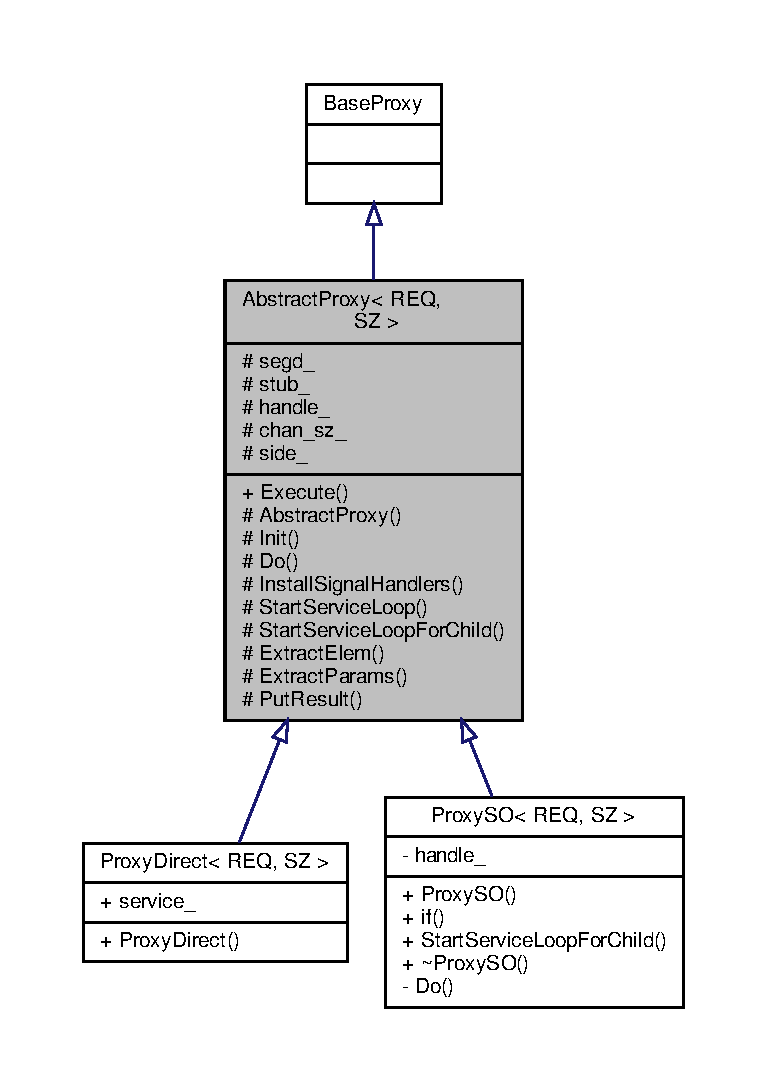
\includegraphics[width=350pt]{classAbstractProxy__inherit__graph}
\end{center}
\end{figure}


Collaboration diagram for Abstract\+Proxy$<$ R\+EQ, SZ $>$\+:
\nopagebreak
\begin{figure}[H]
\begin{center}
\leavevmode
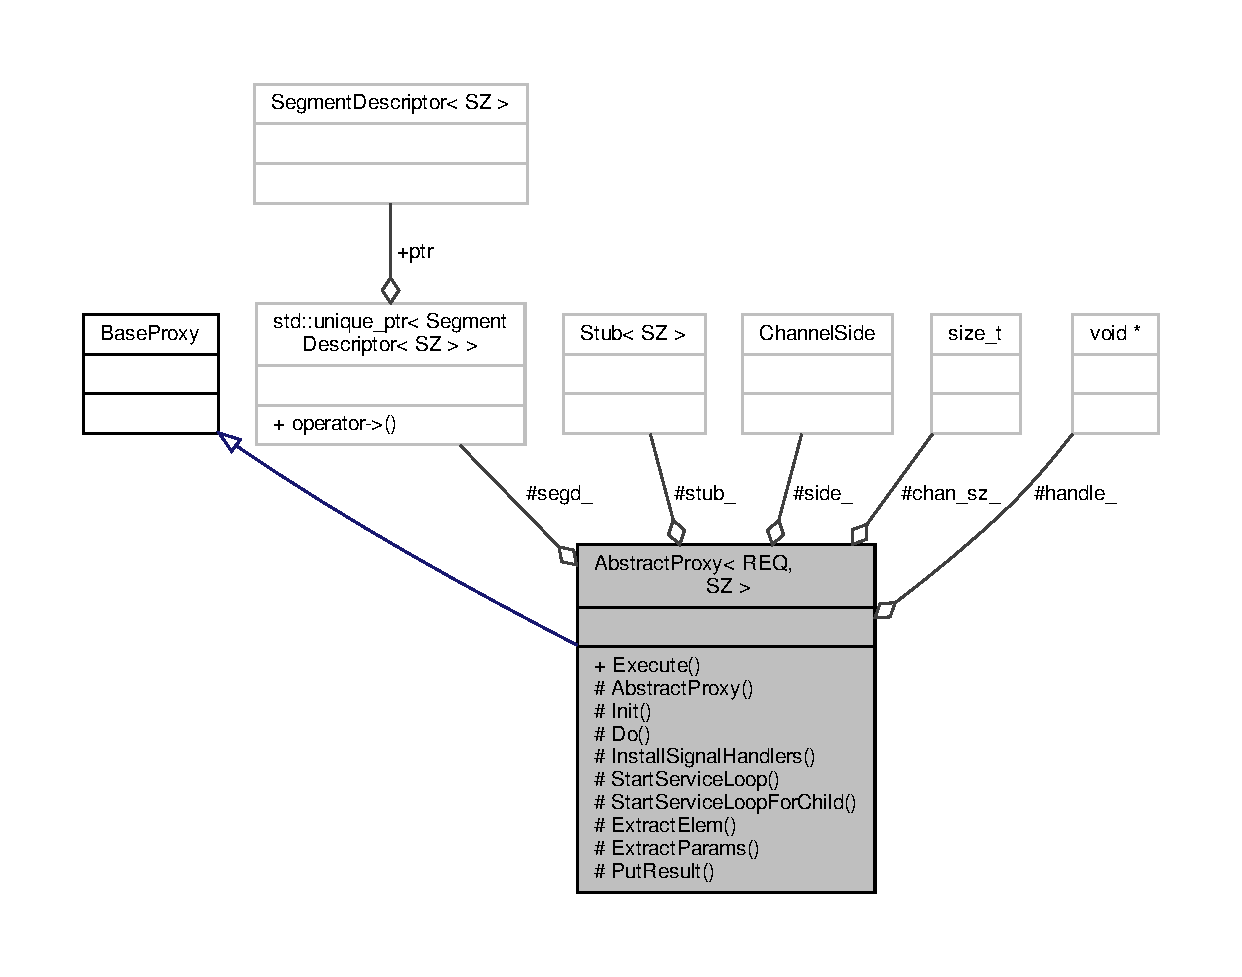
\includegraphics[width=350pt]{classAbstractProxy__coll__graph}
\end{center}
\end{figure}
\subsection*{Public Member Functions}
\begin{DoxyCompactItemize}
\item 
{\footnotesize template$<$typename... Args$>$ }\\\hyperlink{classAbstractProxy_ab2af611a27c14916a27d0e9249f0291b}{R\+ET} \hyperlink{classAbstractProxy_ad1aecd99b6f9da7cbe0c2977f4462040}{Execute} (Args... args)
\end{DoxyCompactItemize}
\subsection*{Protected Types}
\begin{DoxyCompactItemize}
\item 
using \hyperlink{classAbstractProxy_ab2af611a27c14916a27d0e9249f0291b}{R\+ET} = std\+::tuple\+\_\+element\+\_\+t$<$ 0, R\+EQ $>$
\end{DoxyCompactItemize}
\subsection*{Protected Member Functions}
\begin{DoxyCompactItemize}
\item 
\hyperlink{classAbstractProxy_a7ab9f653b68797bbd32b6ed90116ca9d}{Abstract\+Proxy} ()
\item 
void \hyperlink{classAbstractProxy_a9d411fc2a8ff05b6cbf47b2152578e2a}{Init} ()
\item 
virtual void \hyperlink{classAbstractProxy_ab772bf6acfc0b7f69eae6fcc4039df8d}{Do} (R\+EQ \&)=0
\item 
void \hyperlink{classAbstractProxy_a9f368f0e76ba153626f0db982ebe389c}{Install\+Signal\+Handlers} ()
\item 
void \hyperlink{classAbstractProxy_ae0ce7181a041a8845a114f7f1c6768bf}{Start\+Service\+Loop} ()
\item 
void \hyperlink{classAbstractProxy_a8e4f4208efe95831a8bdb4cf139ec0f7}{Start\+Service\+Loop\+For\+Child} ()
\item 
{\footnotesize template$<$int N, typename T\+UP $>$ }\\void \hyperlink{classAbstractProxy_a71a17de97da68a12f3cc7d23995478e2}{Extract\+Elem} (T\+UP \&instance, void $\ast$\&recv)
\item 
{\footnotesize template$<$typename T $>$ }\\auto \hyperlink{classAbstractProxy_a64cad7553939288e10994b4a7fc2557f}{Extract\+Params} (void $\ast$recv)
\item 
{\footnotesize template$<$typename T $>$ }\\void \hyperlink{classAbstractProxy_ad3f858bad58a93f75984d2d0a5bc9081}{Put\+Result} (T \&tup, void $\ast$snd)
\end{DoxyCompactItemize}
\subsection*{Protected Attributes}
\begin{DoxyCompactItemize}
\item 
std\+::unique\+\_\+ptr$<$ \hyperlink{classSegmentDescriptor}{Segment\+Descriptor}$<$ SZ $>$ $>$ \hyperlink{classAbstractProxy_a747e1ccbb8314755f6218ab34b29c5cb}{segd\+\_\+}
\item 
\hyperlink{classStub}{Stub}$<$ SZ $>$ \hyperlink{classAbstractProxy_a2436619808b225e493b2e8745158b49d}{stub\+\_\+}
\item 
void $\ast$ \hyperlink{classAbstractProxy_a28c08cb0041452a38092340256ae4e4b}{handle\+\_\+}
\item 
std\+::size\+\_\+t \hyperlink{classAbstractProxy_a42fcfb0f73620c947800c4fca528db6b}{chan\+\_\+sz\+\_\+}
\item 
\hyperlink{proxy_8hpp_a249fda9ad200a554304ecf8de90d6877}{Channel\+Side} \hyperlink{classAbstractProxy_a15f6c1ab1f6a16ac7ba7a2d6e7bf8744}{side\+\_\+}
\end{DoxyCompactItemize}


\subsection{Member Typedef Documentation}
\mbox{\Hypertarget{classAbstractProxy_ab2af611a27c14916a27d0e9249f0291b}\label{classAbstractProxy_ab2af611a27c14916a27d0e9249f0291b}} 
\index{Abstract\+Proxy@{Abstract\+Proxy}!R\+ET@{R\+ET}}
\index{R\+ET@{R\+ET}!Abstract\+Proxy@{Abstract\+Proxy}}
\subsubsection{\texorpdfstring{R\+ET}{RET}}
{\footnotesize\ttfamily template$<$typename R\+EQ, std\+::size\+\_\+t SZ$>$ \\
using \hyperlink{classAbstractProxy}{Abstract\+Proxy}$<$ R\+EQ, SZ $>$\+::\hyperlink{classAbstractProxy_ab2af611a27c14916a27d0e9249f0291b}{R\+ET} =  std\+::tuple\+\_\+element\+\_\+t$<$0, R\+EQ$>$\hspace{0.3cm}{\ttfamily [protected]}}



\subsection{Constructor \& Destructor Documentation}
\mbox{\Hypertarget{classAbstractProxy_a7ab9f653b68797bbd32b6ed90116ca9d}\label{classAbstractProxy_a7ab9f653b68797bbd32b6ed90116ca9d}} 
\index{Abstract\+Proxy@{Abstract\+Proxy}!Abstract\+Proxy@{Abstract\+Proxy}}
\index{Abstract\+Proxy@{Abstract\+Proxy}!Abstract\+Proxy@{Abstract\+Proxy}}
\subsubsection{\texorpdfstring{Abstract\+Proxy()}{AbstractProxy()}}
{\footnotesize\ttfamily template$<$typename R\+EQ, std\+::size\+\_\+t SZ$>$ \\
\hyperlink{classAbstractProxy}{Abstract\+Proxy}$<$ R\+EQ, SZ $>$\+::\hyperlink{classAbstractProxy}{Abstract\+Proxy} (\begin{DoxyParamCaption}{ }\end{DoxyParamCaption})\hspace{0.3cm}{\ttfamily [inline]}, {\ttfamily [protected]}}



\subsection{Member Function Documentation}
\mbox{\Hypertarget{classAbstractProxy_ab772bf6acfc0b7f69eae6fcc4039df8d}\label{classAbstractProxy_ab772bf6acfc0b7f69eae6fcc4039df8d}} 
\index{Abstract\+Proxy@{Abstract\+Proxy}!Do@{Do}}
\index{Do@{Do}!Abstract\+Proxy@{Abstract\+Proxy}}
\subsubsection{\texorpdfstring{Do()}{Do()}}
{\footnotesize\ttfamily template$<$typename R\+EQ, std\+::size\+\_\+t SZ$>$ \\
virtual void \hyperlink{classAbstractProxy}{Abstract\+Proxy}$<$ R\+EQ, SZ $>$\+::Do (\begin{DoxyParamCaption}\item[{R\+EQ \&}]{ }\end{DoxyParamCaption})\hspace{0.3cm}{\ttfamily [protected]}, {\ttfamily [pure virtual]}}



Implemented in \hyperlink{classProxySO_aea9532d196e05f80b2dd0de425df711f}{Proxy\+S\+O$<$ R\+E\+Q, S\+Z $>$}.

\mbox{\Hypertarget{classAbstractProxy_ad1aecd99b6f9da7cbe0c2977f4462040}\label{classAbstractProxy_ad1aecd99b6f9da7cbe0c2977f4462040}} 
\index{Abstract\+Proxy@{Abstract\+Proxy}!Execute@{Execute}}
\index{Execute@{Execute}!Abstract\+Proxy@{Abstract\+Proxy}}
\subsubsection{\texorpdfstring{Execute()}{Execute()}}
{\footnotesize\ttfamily template$<$typename R\+EQ, std\+::size\+\_\+t SZ$>$ \\
template$<$typename... Args$>$ \\
\hyperlink{classAbstractProxy_ab2af611a27c14916a27d0e9249f0291b}{R\+ET} \hyperlink{classAbstractProxy}{Abstract\+Proxy}$<$ R\+EQ, SZ $>$\+::Execute (\begin{DoxyParamCaption}\item[{Args...}]{args }\end{DoxyParamCaption})\hspace{0.3cm}{\ttfamily [inline]}}

\mbox{\Hypertarget{classAbstractProxy_a71a17de97da68a12f3cc7d23995478e2}\label{classAbstractProxy_a71a17de97da68a12f3cc7d23995478e2}} 
\index{Abstract\+Proxy@{Abstract\+Proxy}!Extract\+Elem@{Extract\+Elem}}
\index{Extract\+Elem@{Extract\+Elem}!Abstract\+Proxy@{Abstract\+Proxy}}
\subsubsection{\texorpdfstring{Extract\+Elem()}{ExtractElem()}}
{\footnotesize\ttfamily template$<$typename R\+EQ, std\+::size\+\_\+t SZ$>$ \\
template$<$int N, typename T\+UP $>$ \\
void \hyperlink{classAbstractProxy}{Abstract\+Proxy}$<$ R\+EQ, SZ $>$\+::Extract\+Elem (\begin{DoxyParamCaption}\item[{T\+UP \&}]{instance,  }\item[{void $\ast$\&}]{recv }\end{DoxyParamCaption})\hspace{0.3cm}{\ttfamily [inline]}, {\ttfamily [protected]}}

\mbox{\Hypertarget{classAbstractProxy_a64cad7553939288e10994b4a7fc2557f}\label{classAbstractProxy_a64cad7553939288e10994b4a7fc2557f}} 
\index{Abstract\+Proxy@{Abstract\+Proxy}!Extract\+Params@{Extract\+Params}}
\index{Extract\+Params@{Extract\+Params}!Abstract\+Proxy@{Abstract\+Proxy}}
\subsubsection{\texorpdfstring{Extract\+Params()}{ExtractParams()}}
{\footnotesize\ttfamily template$<$typename R\+EQ, std\+::size\+\_\+t SZ$>$ \\
template$<$typename T $>$ \\
auto \hyperlink{classAbstractProxy}{Abstract\+Proxy}$<$ R\+EQ, SZ $>$\+::Extract\+Params (\begin{DoxyParamCaption}\item[{void $\ast$}]{recv }\end{DoxyParamCaption})\hspace{0.3cm}{\ttfamily [inline]}, {\ttfamily [protected]}}

\mbox{\Hypertarget{classAbstractProxy_a9d411fc2a8ff05b6cbf47b2152578e2a}\label{classAbstractProxy_a9d411fc2a8ff05b6cbf47b2152578e2a}} 
\index{Abstract\+Proxy@{Abstract\+Proxy}!Init@{Init}}
\index{Init@{Init}!Abstract\+Proxy@{Abstract\+Proxy}}
\subsubsection{\texorpdfstring{Init()}{Init()}}
{\footnotesize\ttfamily template$<$typename R\+EQ, std\+::size\+\_\+t SZ$>$ \\
void \hyperlink{classAbstractProxy}{Abstract\+Proxy}$<$ R\+EQ, SZ $>$\+::Init (\begin{DoxyParamCaption}{ }\end{DoxyParamCaption})\hspace{0.3cm}{\ttfamily [inline]}, {\ttfamily [protected]}}

\mbox{\Hypertarget{classAbstractProxy_a9f368f0e76ba153626f0db982ebe389c}\label{classAbstractProxy_a9f368f0e76ba153626f0db982ebe389c}} 
\index{Abstract\+Proxy@{Abstract\+Proxy}!Install\+Signal\+Handlers@{Install\+Signal\+Handlers}}
\index{Install\+Signal\+Handlers@{Install\+Signal\+Handlers}!Abstract\+Proxy@{Abstract\+Proxy}}
\subsubsection{\texorpdfstring{Install\+Signal\+Handlers()}{InstallSignalHandlers()}}
{\footnotesize\ttfamily template$<$typename R\+EQ, std\+::size\+\_\+t SZ$>$ \\
void \hyperlink{classAbstractProxy}{Abstract\+Proxy}$<$ R\+EQ, SZ $>$\+::Install\+Signal\+Handlers (\begin{DoxyParamCaption}{ }\end{DoxyParamCaption})\hspace{0.3cm}{\ttfamily [inline]}, {\ttfamily [protected]}}

Here is the call graph for this function\+:
\nopagebreak
\begin{figure}[H]
\begin{center}
\leavevmode
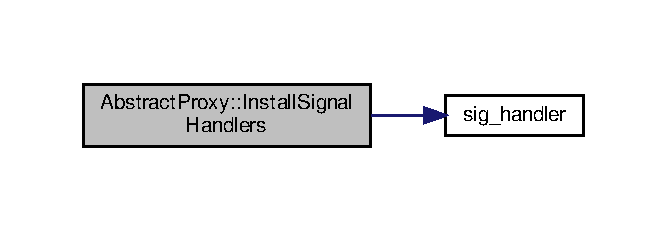
\includegraphics[width=320pt]{classAbstractProxy_a9f368f0e76ba153626f0db982ebe389c_cgraph}
\end{center}
\end{figure}
\mbox{\Hypertarget{classAbstractProxy_ad3f858bad58a93f75984d2d0a5bc9081}\label{classAbstractProxy_ad3f858bad58a93f75984d2d0a5bc9081}} 
\index{Abstract\+Proxy@{Abstract\+Proxy}!Put\+Result@{Put\+Result}}
\index{Put\+Result@{Put\+Result}!Abstract\+Proxy@{Abstract\+Proxy}}
\subsubsection{\texorpdfstring{Put\+Result()}{PutResult()}}
{\footnotesize\ttfamily template$<$typename R\+EQ, std\+::size\+\_\+t SZ$>$ \\
template$<$typename T $>$ \\
void \hyperlink{classAbstractProxy}{Abstract\+Proxy}$<$ R\+EQ, SZ $>$\+::Put\+Result (\begin{DoxyParamCaption}\item[{T \&}]{tup,  }\item[{void $\ast$}]{snd }\end{DoxyParamCaption})\hspace{0.3cm}{\ttfamily [inline]}, {\ttfamily [protected]}}

\mbox{\Hypertarget{classAbstractProxy_ae0ce7181a041a8845a114f7f1c6768bf}\label{classAbstractProxy_ae0ce7181a041a8845a114f7f1c6768bf}} 
\index{Abstract\+Proxy@{Abstract\+Proxy}!Start\+Service\+Loop@{Start\+Service\+Loop}}
\index{Start\+Service\+Loop@{Start\+Service\+Loop}!Abstract\+Proxy@{Abstract\+Proxy}}
\subsubsection{\texorpdfstring{Start\+Service\+Loop()}{StartServiceLoop()}}
{\footnotesize\ttfamily template$<$typename R\+EQ, std\+::size\+\_\+t SZ$>$ \\
void \hyperlink{classAbstractProxy}{Abstract\+Proxy}$<$ R\+EQ, SZ $>$\+::Start\+Service\+Loop (\begin{DoxyParamCaption}{ }\end{DoxyParamCaption})\hspace{0.3cm}{\ttfamily [inline]}, {\ttfamily [protected]}}

\mbox{\Hypertarget{classAbstractProxy_a8e4f4208efe95831a8bdb4cf139ec0f7}\label{classAbstractProxy_a8e4f4208efe95831a8bdb4cf139ec0f7}} 
\index{Abstract\+Proxy@{Abstract\+Proxy}!Start\+Service\+Loop\+For\+Child@{Start\+Service\+Loop\+For\+Child}}
\index{Start\+Service\+Loop\+For\+Child@{Start\+Service\+Loop\+For\+Child}!Abstract\+Proxy@{Abstract\+Proxy}}
\subsubsection{\texorpdfstring{Start\+Service\+Loop\+For\+Child()}{StartServiceLoopForChild()}}
{\footnotesize\ttfamily template$<$typename R\+EQ, std\+::size\+\_\+t SZ$>$ \\
void \hyperlink{classAbstractProxy}{Abstract\+Proxy}$<$ R\+EQ, SZ $>$\+::Start\+Service\+Loop\+For\+Child (\begin{DoxyParamCaption}{ }\end{DoxyParamCaption})\hspace{0.3cm}{\ttfamily [inline]}, {\ttfamily [protected]}}



\subsection{Member Data Documentation}
\mbox{\Hypertarget{classAbstractProxy_a42fcfb0f73620c947800c4fca528db6b}\label{classAbstractProxy_a42fcfb0f73620c947800c4fca528db6b}} 
\index{Abstract\+Proxy@{Abstract\+Proxy}!chan\+\_\+sz\+\_\+@{chan\+\_\+sz\+\_\+}}
\index{chan\+\_\+sz\+\_\+@{chan\+\_\+sz\+\_\+}!Abstract\+Proxy@{Abstract\+Proxy}}
\subsubsection{\texorpdfstring{chan\+\_\+sz\+\_\+}{chan\_sz\_}}
{\footnotesize\ttfamily template$<$typename R\+EQ, std\+::size\+\_\+t SZ$>$ \\
std\+::size\+\_\+t \hyperlink{classAbstractProxy}{Abstract\+Proxy}$<$ R\+EQ, SZ $>$\+::chan\+\_\+sz\+\_\+\hspace{0.3cm}{\ttfamily [protected]}}

\mbox{\Hypertarget{classAbstractProxy_a28c08cb0041452a38092340256ae4e4b}\label{classAbstractProxy_a28c08cb0041452a38092340256ae4e4b}} 
\index{Abstract\+Proxy@{Abstract\+Proxy}!handle\+\_\+@{handle\+\_\+}}
\index{handle\+\_\+@{handle\+\_\+}!Abstract\+Proxy@{Abstract\+Proxy}}
\subsubsection{\texorpdfstring{handle\+\_\+}{handle\_}}
{\footnotesize\ttfamily template$<$typename R\+EQ, std\+::size\+\_\+t SZ$>$ \\
void$\ast$ \hyperlink{classAbstractProxy}{Abstract\+Proxy}$<$ R\+EQ, SZ $>$\+::handle\+\_\+\hspace{0.3cm}{\ttfamily [protected]}}

\mbox{\Hypertarget{classAbstractProxy_a747e1ccbb8314755f6218ab34b29c5cb}\label{classAbstractProxy_a747e1ccbb8314755f6218ab34b29c5cb}} 
\index{Abstract\+Proxy@{Abstract\+Proxy}!segd\+\_\+@{segd\+\_\+}}
\index{segd\+\_\+@{segd\+\_\+}!Abstract\+Proxy@{Abstract\+Proxy}}
\subsubsection{\texorpdfstring{segd\+\_\+}{segd\_}}
{\footnotesize\ttfamily template$<$typename R\+EQ, std\+::size\+\_\+t SZ$>$ \\
std\+::unique\+\_\+ptr$<$\hyperlink{classSegmentDescriptor}{Segment\+Descriptor}$<$SZ$>$ $>$ \hyperlink{classAbstractProxy}{Abstract\+Proxy}$<$ R\+EQ, SZ $>$\+::segd\+\_\+\hspace{0.3cm}{\ttfamily [protected]}}

\mbox{\Hypertarget{classAbstractProxy_a15f6c1ab1f6a16ac7ba7a2d6e7bf8744}\label{classAbstractProxy_a15f6c1ab1f6a16ac7ba7a2d6e7bf8744}} 
\index{Abstract\+Proxy@{Abstract\+Proxy}!side\+\_\+@{side\+\_\+}}
\index{side\+\_\+@{side\+\_\+}!Abstract\+Proxy@{Abstract\+Proxy}}
\subsubsection{\texorpdfstring{side\+\_\+}{side\_}}
{\footnotesize\ttfamily template$<$typename R\+EQ, std\+::size\+\_\+t SZ$>$ \\
\hyperlink{proxy_8hpp_a249fda9ad200a554304ecf8de90d6877}{Channel\+Side} \hyperlink{classAbstractProxy}{Abstract\+Proxy}$<$ R\+EQ, SZ $>$\+::side\+\_\+\hspace{0.3cm}{\ttfamily [protected]}}

\mbox{\Hypertarget{classAbstractProxy_a2436619808b225e493b2e8745158b49d}\label{classAbstractProxy_a2436619808b225e493b2e8745158b49d}} 
\index{Abstract\+Proxy@{Abstract\+Proxy}!stub\+\_\+@{stub\+\_\+}}
\index{stub\+\_\+@{stub\+\_\+}!Abstract\+Proxy@{Abstract\+Proxy}}
\subsubsection{\texorpdfstring{stub\+\_\+}{stub\_}}
{\footnotesize\ttfamily template$<$typename R\+EQ, std\+::size\+\_\+t SZ$>$ \\
\hyperlink{classStub}{Stub}$<$SZ$>$ \hyperlink{classAbstractProxy}{Abstract\+Proxy}$<$ R\+EQ, SZ $>$\+::stub\+\_\+\hspace{0.3cm}{\ttfamily [protected]}}



The documentation for this class was generated from the following file\+:\begin{DoxyCompactItemize}
\item 
include/\hyperlink{proxy_8hpp}{proxy.\+hpp}\end{DoxyCompactItemize}

\hypertarget{classBaseProxy}{}\section{Base\+Proxy Class Reference}
\label{classBaseProxy}\index{Base\+Proxy@{Base\+Proxy}}


{\ttfamily \#include $<$proxy.\+hpp$>$}



Inheritance diagram for Base\+Proxy\+:
\nopagebreak
\begin{figure}[H]
\begin{center}
\leavevmode
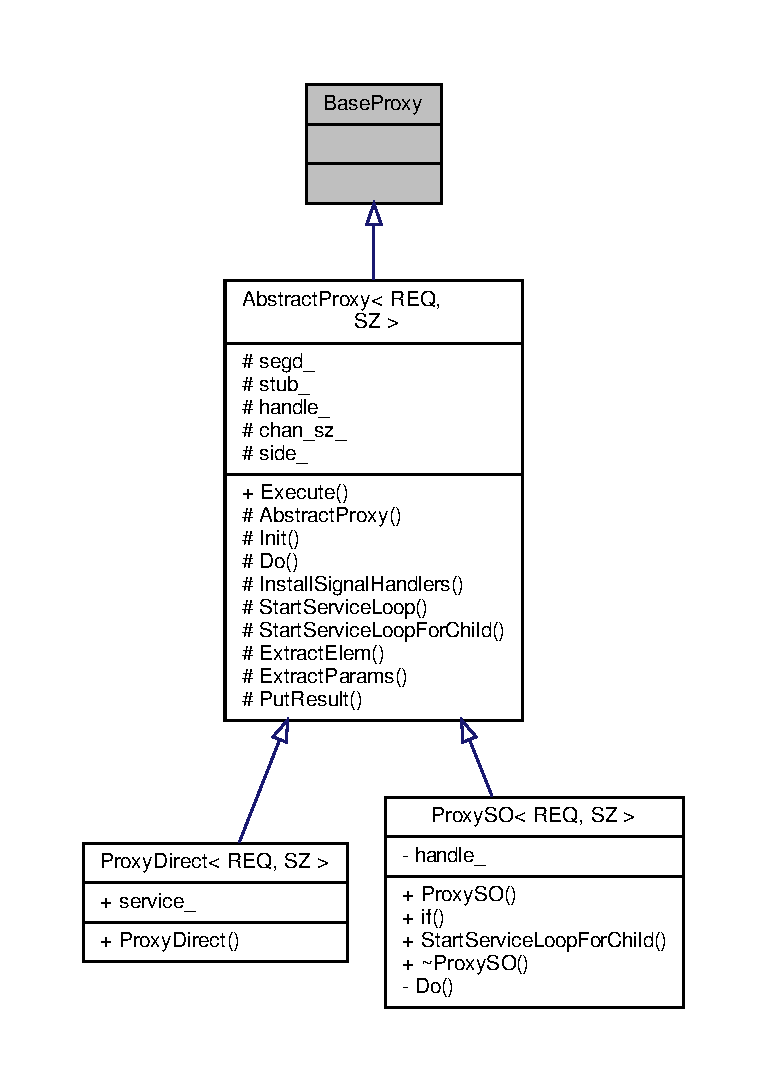
\includegraphics[width=350pt]{classBaseProxy__inherit__graph}
\end{center}
\end{figure}


Collaboration diagram for Base\+Proxy\+:
\nopagebreak
\begin{figure}[H]
\begin{center}
\leavevmode
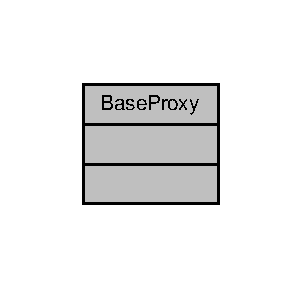
\includegraphics[width=145pt]{classBaseProxy__coll__graph}
\end{center}
\end{figure}


The documentation for this class was generated from the following file\+:\begin{DoxyCompactItemize}
\item 
include/\hyperlink{proxy_8hpp}{proxy.\+hpp}\end{DoxyCompactItemize}

\hypertarget{classChannel}{}\section{Channel$<$ SZ $>$ Class Template Reference}
\label{classChannel}\index{Channel$<$ S\+Z $>$@{Channel$<$ S\+Z $>$}}


{\ttfamily \#include $<$proxy.\+hpp$>$}



Collaboration diagram for Channel$<$ SZ $>$\+:
\nopagebreak
\begin{figure}[H]
\begin{center}
\leavevmode
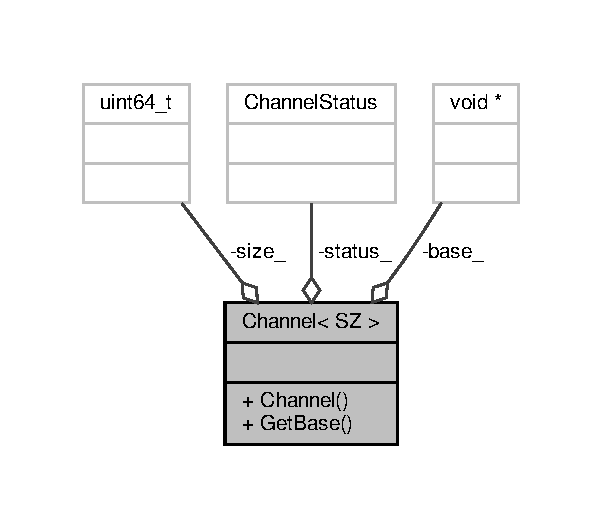
\includegraphics[width=289pt]{classChannel__coll__graph}
\end{center}
\end{figure}
\subsection*{Public Member Functions}
\begin{DoxyCompactItemize}
\item 
\hyperlink{classChannel_a5e18f101c74be5001d6b34a3026c6f7c}{Channel} (std\+::size\+\_\+t sz)
\item 
void $\ast$ \hyperlink{classChannel_a0bfa9c9c5280c8d3776c2e468f63586b}{Get\+Base} ()
\end{DoxyCompactItemize}
\subsection*{Private Attributes}
\begin{DoxyCompactItemize}
\item 
uint64\+\_\+t \hyperlink{classChannel_a7593f310eba67835f7df73f5afdf44e6}{size\+\_\+}
\item 
void $\ast$ \hyperlink{classChannel_a519cfe913cf0fb5b4c3adfa5df29d40c}{base\+\_\+}
\item 
\hyperlink{proxy_8hpp_abdf990fbe51b4c9d3fdcc2fc3c6f9219}{Channel\+Status} \hyperlink{classChannel_a62d282a44d5b5998c0b4fe8299ee1edd}{status\+\_\+}
\end{DoxyCompactItemize}
\subsection*{Friends}
\begin{DoxyCompactItemize}
\item 
class \hyperlink{classChannel_aa9880fe41382d4118e3f013f9058746d}{Segment\+Descriptor$<$ S\+Z $>$}
\end{DoxyCompactItemize}


\subsection{Constructor \& Destructor Documentation}
\mbox{\Hypertarget{classChannel_a5e18f101c74be5001d6b34a3026c6f7c}\label{classChannel_a5e18f101c74be5001d6b34a3026c6f7c}} 
\index{Channel@{Channel}!Channel@{Channel}}
\index{Channel@{Channel}!Channel@{Channel}}
\subsubsection{\texorpdfstring{Channel()}{Channel()}}
{\footnotesize\ttfamily template$<$std\+::size\+\_\+t SZ$>$ \\
\hyperlink{classChannel}{Channel}$<$ SZ $>$\+::\hyperlink{classChannel}{Channel} (\begin{DoxyParamCaption}\item[{std\+::size\+\_\+t}]{sz }\end{DoxyParamCaption})\hspace{0.3cm}{\ttfamily [inline]}}



\subsection{Member Function Documentation}
\mbox{\Hypertarget{classChannel_a0bfa9c9c5280c8d3776c2e468f63586b}\label{classChannel_a0bfa9c9c5280c8d3776c2e468f63586b}} 
\index{Channel@{Channel}!Get\+Base@{Get\+Base}}
\index{Get\+Base@{Get\+Base}!Channel@{Channel}}
\subsubsection{\texorpdfstring{Get\+Base()}{GetBase()}}
{\footnotesize\ttfamily template$<$std\+::size\+\_\+t SZ$>$ \\
void$\ast$ \hyperlink{classChannel}{Channel}$<$ SZ $>$\+::Get\+Base (\begin{DoxyParamCaption}{ }\end{DoxyParamCaption})\hspace{0.3cm}{\ttfamily [inline]}}



\subsection{Friends And Related Function Documentation}
\mbox{\Hypertarget{classChannel_aa9880fe41382d4118e3f013f9058746d}\label{classChannel_aa9880fe41382d4118e3f013f9058746d}} 
\index{Channel@{Channel}!Segment\+Descriptor$<$ S\+Z $>$@{Segment\+Descriptor$<$ S\+Z $>$}}
\index{Segment\+Descriptor$<$ S\+Z $>$@{Segment\+Descriptor$<$ S\+Z $>$}!Channel@{Channel}}
\subsubsection{\texorpdfstring{Segment\+Descriptor$<$ S\+Z $>$}{SegmentDescriptor< SZ >}}
{\footnotesize\ttfamily template$<$std\+::size\+\_\+t SZ$>$ \\
friend class \hyperlink{classSegmentDescriptor}{Segment\+Descriptor}$<$ SZ $>$\hspace{0.3cm}{\ttfamily [friend]}}



\subsection{Member Data Documentation}
\mbox{\Hypertarget{classChannel_a519cfe913cf0fb5b4c3adfa5df29d40c}\label{classChannel_a519cfe913cf0fb5b4c3adfa5df29d40c}} 
\index{Channel@{Channel}!base\+\_\+@{base\+\_\+}}
\index{base\+\_\+@{base\+\_\+}!Channel@{Channel}}
\subsubsection{\texorpdfstring{base\+\_\+}{base\_}}
{\footnotesize\ttfamily template$<$std\+::size\+\_\+t SZ$>$ \\
void$\ast$ \hyperlink{classChannel}{Channel}$<$ SZ $>$\+::base\+\_\+\hspace{0.3cm}{\ttfamily [private]}}

\mbox{\Hypertarget{classChannel_a7593f310eba67835f7df73f5afdf44e6}\label{classChannel_a7593f310eba67835f7df73f5afdf44e6}} 
\index{Channel@{Channel}!size\+\_\+@{size\+\_\+}}
\index{size\+\_\+@{size\+\_\+}!Channel@{Channel}}
\subsubsection{\texorpdfstring{size\+\_\+}{size\_}}
{\footnotesize\ttfamily template$<$std\+::size\+\_\+t SZ$>$ \\
uint64\+\_\+t \hyperlink{classChannel}{Channel}$<$ SZ $>$\+::size\+\_\+\hspace{0.3cm}{\ttfamily [private]}}

\mbox{\Hypertarget{classChannel_a62d282a44d5b5998c0b4fe8299ee1edd}\label{classChannel_a62d282a44d5b5998c0b4fe8299ee1edd}} 
\index{Channel@{Channel}!status\+\_\+@{status\+\_\+}}
\index{status\+\_\+@{status\+\_\+}!Channel@{Channel}}
\subsubsection{\texorpdfstring{status\+\_\+}{status\_}}
{\footnotesize\ttfamily template$<$std\+::size\+\_\+t SZ$>$ \\
\hyperlink{proxy_8hpp_abdf990fbe51b4c9d3fdcc2fc3c6f9219}{Channel\+Status} \hyperlink{classChannel}{Channel}$<$ SZ $>$\+::status\+\_\+\hspace{0.3cm}{\ttfamily [private]}}



The documentation for this class was generated from the following file\+:\begin{DoxyCompactItemize}
\item 
include/\hyperlink{proxy_8hpp}{proxy.\+hpp}\end{DoxyCompactItemize}

\hypertarget{classChildTerminated}{}\section{Child\+Terminated Class Reference}
\label{classChildTerminated}\index{Child\+Terminated@{Child\+Terminated}}


{\ttfamily \#include $<$proxy.\+hpp$>$}



Inheritance diagram for Child\+Terminated\+:
\nopagebreak
\begin{figure}[H]
\begin{center}
\leavevmode
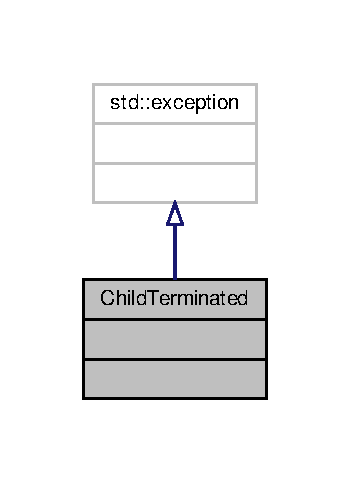
\includegraphics[width=168pt]{classChildTerminated__inherit__graph}
\end{center}
\end{figure}


Collaboration diagram for Child\+Terminated\+:
\nopagebreak
\begin{figure}[H]
\begin{center}
\leavevmode
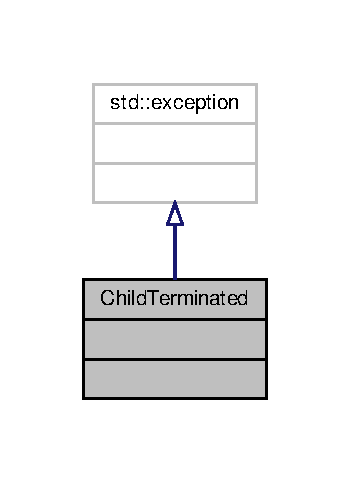
\includegraphics[width=168pt]{classChildTerminated__coll__graph}
\end{center}
\end{figure}


The documentation for this class was generated from the following file\+:\begin{DoxyCompactItemize}
\item 
include/\hyperlink{proxy_8hpp}{proxy.\+hpp}\end{DoxyCompactItemize}

\hypertarget{classOperationFailed}{}\section{Operation\+Failed Class Reference}
\label{classOperationFailed}\index{Operation\+Failed@{Operation\+Failed}}


{\ttfamily \#include $<$proxy.\+hpp$>$}



Inheritance diagram for Operation\+Failed\+:
\nopagebreak
\begin{figure}[H]
\begin{center}
\leavevmode
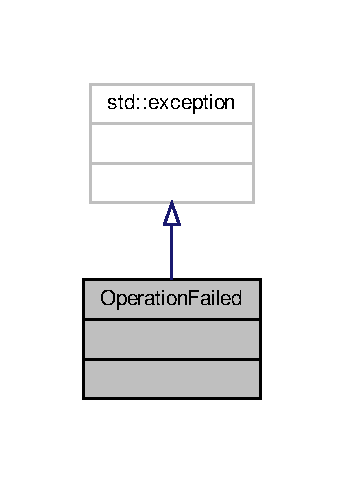
\includegraphics[width=165pt]{classOperationFailed__inherit__graph}
\end{center}
\end{figure}


Collaboration diagram for Operation\+Failed\+:
\nopagebreak
\begin{figure}[H]
\begin{center}
\leavevmode
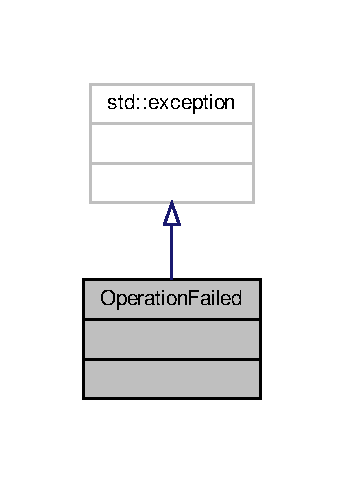
\includegraphics[width=165pt]{classOperationFailed__coll__graph}
\end{center}
\end{figure}


The documentation for this class was generated from the following file\+:\begin{DoxyCompactItemize}
\item 
include/\hyperlink{proxy_8hpp}{proxy.\+hpp}\end{DoxyCompactItemize}

\hypertarget{classParentTerminated}{}\section{Parent\+Terminated Class Reference}
\label{classParentTerminated}\index{Parent\+Terminated@{Parent\+Terminated}}


{\ttfamily \#include $<$proxy.\+hpp$>$}



Inheritance diagram for Parent\+Terminated\+:
\nopagebreak
\begin{figure}[H]
\begin{center}
\leavevmode
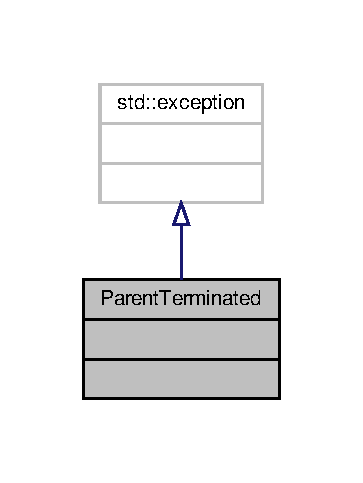
\includegraphics[width=174pt]{classParentTerminated__inherit__graph}
\end{center}
\end{figure}


Collaboration diagram for Parent\+Terminated\+:
\nopagebreak
\begin{figure}[H]
\begin{center}
\leavevmode
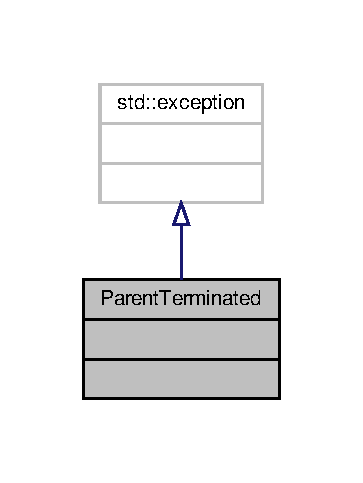
\includegraphics[width=174pt]{classParentTerminated__coll__graph}
\end{center}
\end{figure}


The documentation for this class was generated from the following file\+:\begin{DoxyCompactItemize}
\item 
include/\hyperlink{proxy_8hpp}{proxy.\+hpp}\end{DoxyCompactItemize}

\hypertarget{classProxy}{}\section{Proxy$<$ R\+EQ, SZ, S\+E\+RV $>$ Class Template Reference}
\label{classProxy}\index{Proxy$<$ R\+E\+Q, S\+Z, S\+E\+R\+V $>$@{Proxy$<$ R\+E\+Q, S\+Z, S\+E\+R\+V $>$}}


{\ttfamily \#include $<$proxy.\+hpp$>$}



Collaboration diagram for Proxy$<$ R\+EQ, SZ, S\+E\+RV $>$\+:
\nopagebreak
\begin{figure}[H]
\begin{center}
\leavevmode
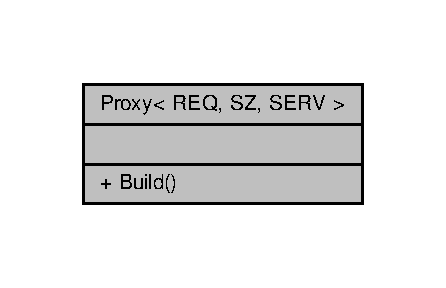
\includegraphics[width=214pt]{classProxy__coll__graph}
\end{center}
\end{figure}
\subsection*{Static Public Member Functions}
\begin{DoxyCompactItemize}
\item 
{\footnotesize template$<$typename... Args$>$ }\\static decltype(auto) \hyperlink{classProxy_a06fe8fe4b6011f5bb4efbe3d7552939a}{Build} (Args... args)
\end{DoxyCompactItemize}


\subsection{Member Function Documentation}
\mbox{\Hypertarget{classProxy_a06fe8fe4b6011f5bb4efbe3d7552939a}\label{classProxy_a06fe8fe4b6011f5bb4efbe3d7552939a}} 
\index{Proxy@{Proxy}!Build@{Build}}
\index{Build@{Build}!Proxy@{Proxy}}
\subsubsection{\texorpdfstring{Build()}{Build()}}
{\footnotesize\ttfamily template$<$typename R\+EQ , std\+::size\+\_\+t SZ = 4096, template$<$ typename $>$ class S\+E\+RV = std\+::void\+\_\+t$>$ \\
template$<$typename... Args$>$ \\
static decltype(auto) \hyperlink{classProxy}{Proxy}$<$ R\+EQ, SZ, S\+E\+RV $>$\+::Build (\begin{DoxyParamCaption}\item[{Args...}]{args }\end{DoxyParamCaption})\hspace{0.3cm}{\ttfamily [inline]}, {\ttfamily [static]}}



The documentation for this class was generated from the following file\+:\begin{DoxyCompactItemize}
\item 
include/\hyperlink{proxy_8hpp}{proxy.\+hpp}\end{DoxyCompactItemize}

\hypertarget{classProxyDirect}{}\section{Proxy\+Direct$<$ R\+EQ, SZ, S\+E\+RV $>$ Class Template Reference}
\label{classProxyDirect}\index{Proxy\+Direct$<$ R\+E\+Q, S\+Z, S\+E\+R\+V $>$@{Proxy\+Direct$<$ R\+E\+Q, S\+Z, S\+E\+R\+V $>$}}


{\ttfamily \#include $<$proxy.\+hpp$>$}



Inheritance diagram for Proxy\+Direct$<$ R\+EQ, SZ, S\+E\+RV $>$\+:
\nopagebreak
\begin{figure}[H]
\begin{center}
\leavevmode
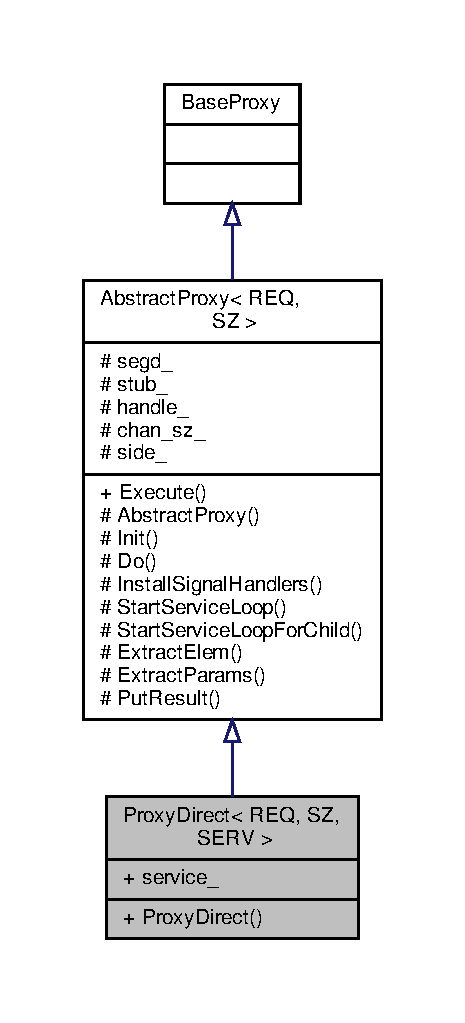
\includegraphics[width=223pt]{classProxyDirect__inherit__graph}
\end{center}
\end{figure}


Collaboration diagram for Proxy\+Direct$<$ R\+EQ, SZ, S\+E\+RV $>$\+:
\nopagebreak
\begin{figure}[H]
\begin{center}
\leavevmode
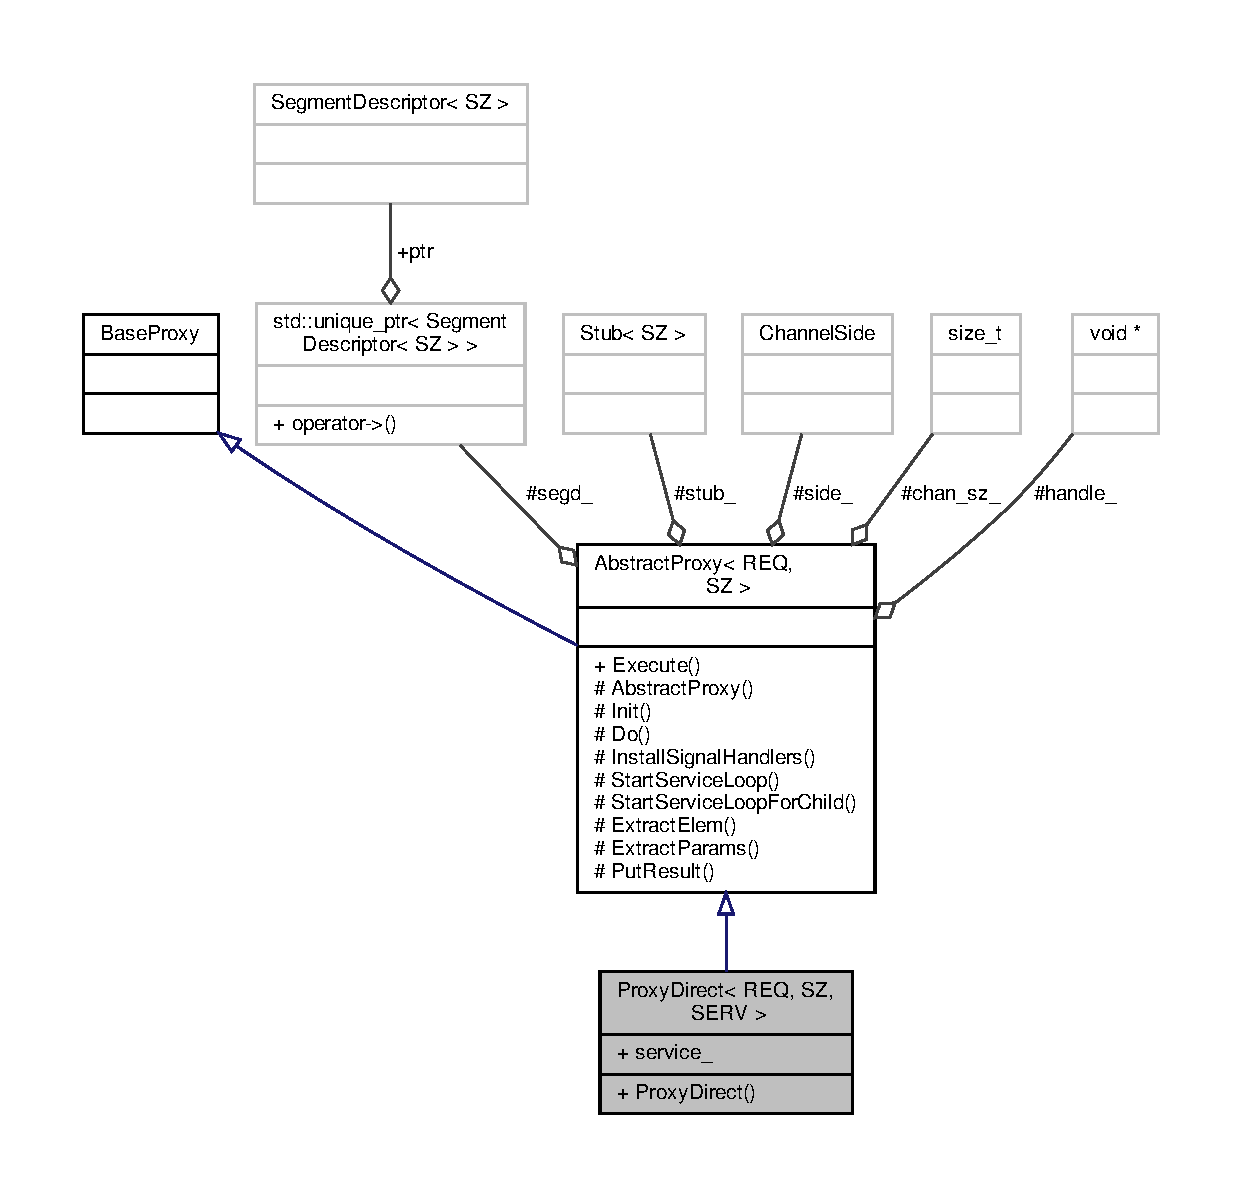
\includegraphics[width=350pt]{classProxyDirect__coll__graph}
\end{center}
\end{figure}
\subsection*{Public Types}
\begin{DoxyCompactItemize}
\item 
using \hyperlink{classProxyDirect_a7ea817de80b380e39bdf58a9ef25726a}{R\+ET} = typename \hyperlink{classAbstractProxy}{Abstract\+Proxy}$<$ R\+EQ, SZ $>$\+::\hyperlink{classAbstractProxy_ab2af611a27c14916a27d0e9249f0291b}{R\+ET}
\end{DoxyCompactItemize}
\subsection*{Public Member Functions}
\begin{DoxyCompactItemize}
\item 
\hyperlink{classProxyDirect_a2c7e97bb43a6418010031f7aa9c5d79b}{Proxy\+Direct} ()
\end{DoxyCompactItemize}
\subsection*{Public Attributes}
\begin{DoxyCompactItemize}
\item 
\hyperlink{classProxyDirect_a2c2d9a268b533d24d49b27f999583910}{service\+\_\+}
\end{DoxyCompactItemize}
\subsection*{Additional Inherited Members}


\subsection{Member Typedef Documentation}
\mbox{\Hypertarget{classProxyDirect_a7ea817de80b380e39bdf58a9ef25726a}\label{classProxyDirect_a7ea817de80b380e39bdf58a9ef25726a}} 
\index{Proxy\+Direct@{Proxy\+Direct}!R\+ET@{R\+ET}}
\index{R\+ET@{R\+ET}!Proxy\+Direct@{Proxy\+Direct}}
\subsubsection{\texorpdfstring{R\+ET}{RET}}
{\footnotesize\ttfamily template$<$typename R\+EQ , std\+::size\+\_\+t SZ, template$<$ typename $>$ class S\+E\+RV$>$ \\
using \hyperlink{classProxyDirect}{Proxy\+Direct}$<$ R\+EQ, SZ, S\+E\+RV $>$\+::\hyperlink{classAbstractProxy_ab2af611a27c14916a27d0e9249f0291b}{R\+ET} =  typename \hyperlink{classAbstractProxy}{Abstract\+Proxy}$<$R\+EQ, SZ$>$\+::\hyperlink{classAbstractProxy_ab2af611a27c14916a27d0e9249f0291b}{R\+ET}}



\subsection{Constructor \& Destructor Documentation}
\mbox{\Hypertarget{classProxyDirect_a2c7e97bb43a6418010031f7aa9c5d79b}\label{classProxyDirect_a2c7e97bb43a6418010031f7aa9c5d79b}} 
\index{Proxy\+Direct@{Proxy\+Direct}!Proxy\+Direct@{Proxy\+Direct}}
\index{Proxy\+Direct@{Proxy\+Direct}!Proxy\+Direct@{Proxy\+Direct}}
\subsubsection{\texorpdfstring{Proxy\+Direct()}{ProxyDirect()}}
{\footnotesize\ttfamily template$<$typename R\+EQ , std\+::size\+\_\+t SZ, template$<$ typename $>$ class S\+E\+RV$>$ \\
\hyperlink{classProxyDirect}{Proxy\+Direct}$<$ R\+EQ, SZ, S\+E\+RV $>$\+::\hyperlink{classProxyDirect}{Proxy\+Direct} (\begin{DoxyParamCaption}{ }\end{DoxyParamCaption})\hspace{0.3cm}{\ttfamily [inline]}}



\subsection{Member Data Documentation}
\mbox{\Hypertarget{classProxyDirect_a2c2d9a268b533d24d49b27f999583910}\label{classProxyDirect_a2c2d9a268b533d24d49b27f999583910}} 
\index{Proxy\+Direct@{Proxy\+Direct}!service\+\_\+@{service\+\_\+}}
\index{service\+\_\+@{service\+\_\+}!Proxy\+Direct@{Proxy\+Direct}}
\subsubsection{\texorpdfstring{service\+\_\+}{service\_}}
{\footnotesize\ttfamily template$<$typename R\+EQ , std\+::size\+\_\+t SZ, template$<$ typename $>$ class S\+E\+RV$>$ \\
\hyperlink{classProxyDirect}{Proxy\+Direct}$<$ R\+EQ, SZ, S\+E\+RV $>$\+::service\+\_\+}

{\bfseries Initial value\+:}
\begin{DoxyCode}
\{\}
    \{
        this->\hyperlink{classAbstractProxy_a8e4f4208efe95831a8bdb4cf139ec0f7}{StartServiceLoopForChild}();
    \}

    ~\hyperlink{classProxyDirect}{ProxyDirect}()
    \{\}

    \textcolor{keywordtype}{void}
    \hyperlink{classAbstractProxy_ab772bf6acfc0b7f69eae6fcc4039df8d}{Do}(REQ& ins)\textcolor{keyword}{ override}
\textcolor{keyword}{    }\{
        \hyperlink{classProxyDirect_a2c2d9a268b533d24d49b27f999583910}{service\_}.Handle(ins);
    \}

\textcolor{keyword}{private}:
    SERV<REQ> \hyperlink{classProxyDirect_a2c2d9a268b533d24d49b27f999583910}{service\_}
\end{DoxyCode}


The documentation for this class was generated from the following file\+:\begin{DoxyCompactItemize}
\item 
include/\hyperlink{proxy_8hpp}{proxy.\+hpp}\end{DoxyCompactItemize}

\hypertarget{classProxySO}{}\section{Proxy\+SO$<$ R\+EQ, SZ $>$ Class Template Reference}
\label{classProxySO}\index{Proxy\+S\+O$<$ R\+E\+Q, S\+Z $>$@{Proxy\+S\+O$<$ R\+E\+Q, S\+Z $>$}}


{\ttfamily \#include $<$proxy.\+hpp$>$}



Inheritance diagram for Proxy\+SO$<$ R\+EQ, SZ $>$\+:
\nopagebreak
\begin{figure}[H]
\begin{center}
\leavevmode
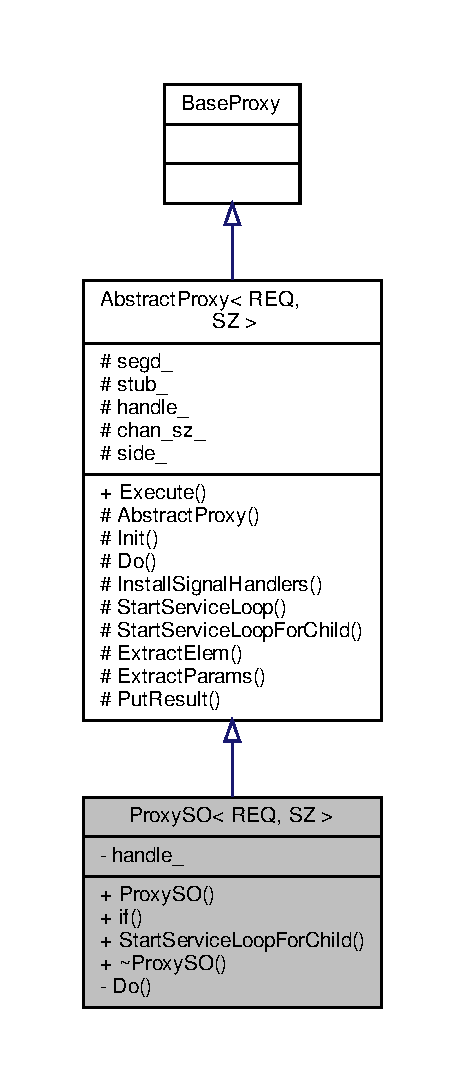
\includegraphics[width=223pt]{classProxySO__inherit__graph}
\end{center}
\end{figure}


Collaboration diagram for Proxy\+SO$<$ R\+EQ, SZ $>$\+:
\nopagebreak
\begin{figure}[H]
\begin{center}
\leavevmode
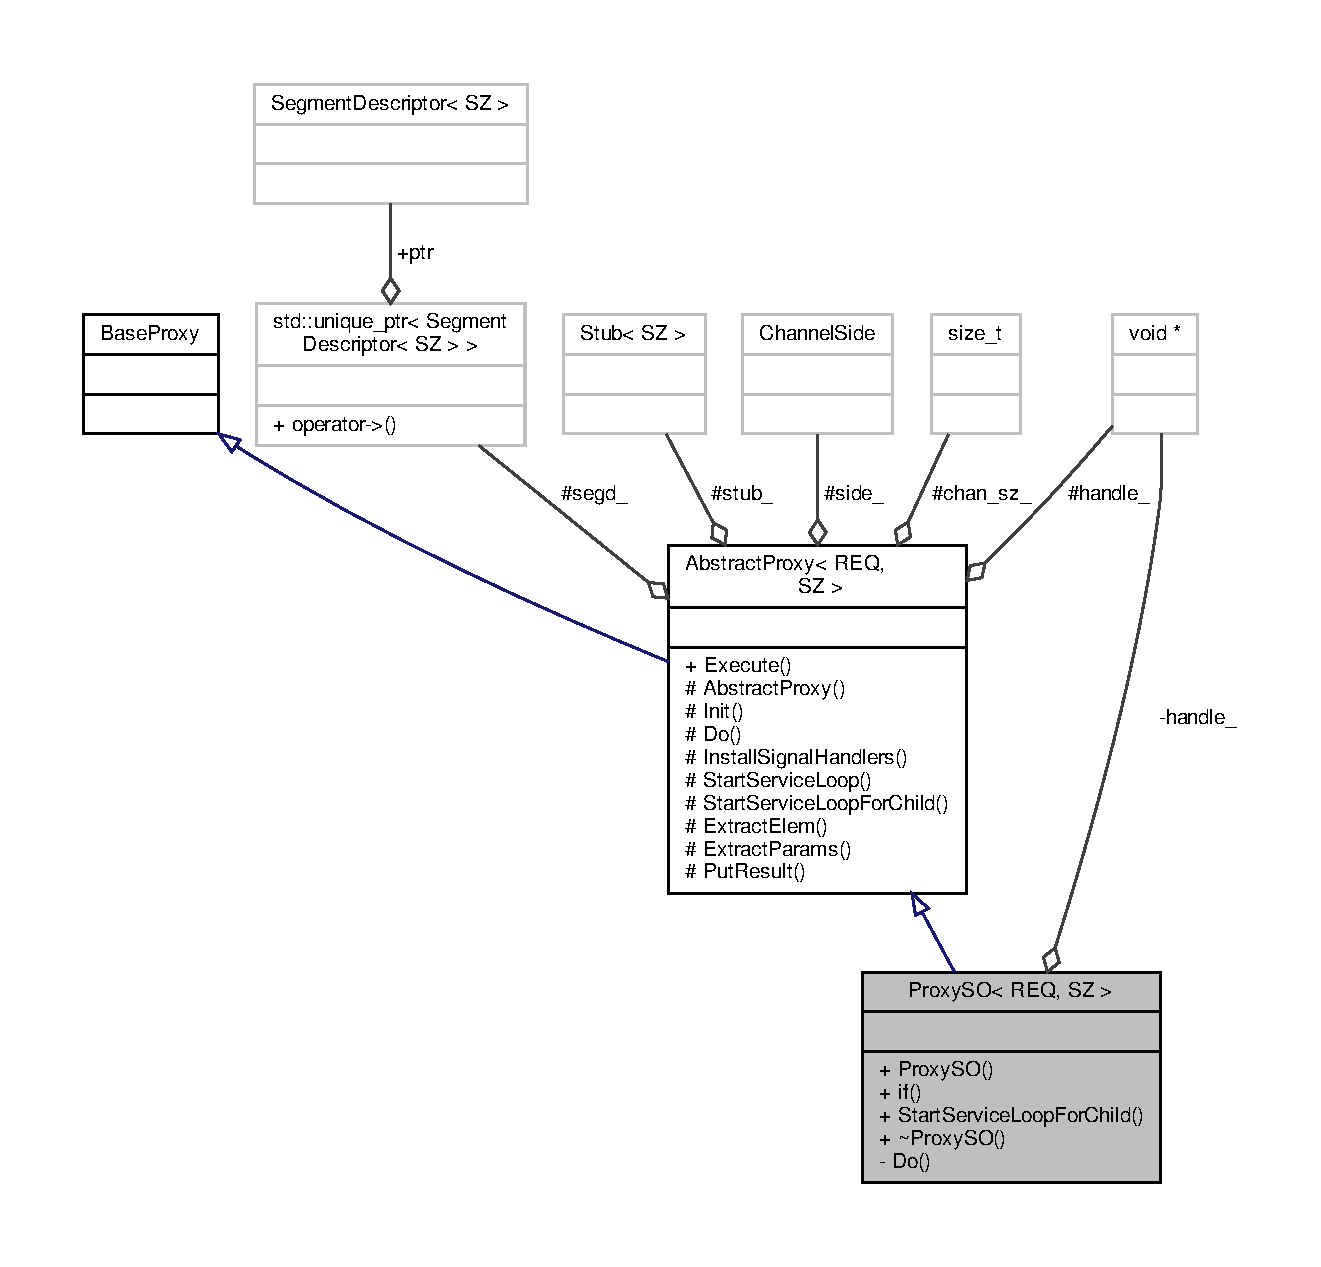
\includegraphics[width=350pt]{classProxySO__coll__graph}
\end{center}
\end{figure}
\subsection*{Public Member Functions}
\begin{DoxyCompactItemize}
\item 
\hyperlink{classProxySO_a75fcf01c02b0aae33be41eea99a8b3e3}{Proxy\+SO} (std\+::string soname)
\item 
\hyperlink{classProxySO_affdd32b972bf9459a0f7ba37ec44a66a}{if} (!\hyperlink{classProxySO_a8db0f87ceb9dc54bd30b212394a74d09}{handle\+\_\+})
\item 
this \hyperlink{classProxySO_a1b036308a00c892930eb4e4955ed4716}{Start\+Service\+Loop\+For\+Child} ()
\item 
\hyperlink{classProxySO_acfe42e6a280ffe394926d16ddd13c3d2}{$\sim$\+Proxy\+SO} ()
\end{DoxyCompactItemize}
\subsection*{Private Types}
\begin{DoxyCompactItemize}
\item 
using \hyperlink{classProxySO_aab633f27d11bc301d3fe6714293cdff9}{R\+ET} = typename \hyperlink{classAbstractProxy}{Abstract\+Proxy}$<$ R\+EQ, SZ $>$\+::\hyperlink{classAbstractProxy_ab2af611a27c14916a27d0e9249f0291b}{R\+ET}
\end{DoxyCompactItemize}
\subsection*{Private Member Functions}
\begin{DoxyCompactItemize}
\item 
void \hyperlink{classProxySO_aea9532d196e05f80b2dd0de425df711f}{Do} (R\+EQ \&ins) override
\end{DoxyCompactItemize}
\subsection*{Private Attributes}
\begin{DoxyCompactItemize}
\item 
void $\ast$ \hyperlink{classProxySO_a8db0f87ceb9dc54bd30b212394a74d09}{handle\+\_\+}
\end{DoxyCompactItemize}
\subsection*{Additional Inherited Members}


\subsection{Member Typedef Documentation}
\mbox{\Hypertarget{classProxySO_aab633f27d11bc301d3fe6714293cdff9}\label{classProxySO_aab633f27d11bc301d3fe6714293cdff9}} 
\index{Proxy\+SO@{Proxy\+SO}!R\+ET@{R\+ET}}
\index{R\+ET@{R\+ET}!Proxy\+SO@{Proxy\+SO}}
\subsubsection{\texorpdfstring{R\+ET}{RET}}
{\footnotesize\ttfamily template$<$typename R\+EQ , std\+::size\+\_\+t SZ$>$ \\
using \hyperlink{classProxySO}{Proxy\+SO}$<$ R\+EQ, SZ $>$\+::\hyperlink{classAbstractProxy_ab2af611a27c14916a27d0e9249f0291b}{R\+ET} =  typename \hyperlink{classAbstractProxy}{Abstract\+Proxy}$<$R\+EQ, SZ$>$\+::\hyperlink{classAbstractProxy_ab2af611a27c14916a27d0e9249f0291b}{R\+ET}\hspace{0.3cm}{\ttfamily [private]}}



\subsection{Constructor \& Destructor Documentation}
\mbox{\Hypertarget{classProxySO_a75fcf01c02b0aae33be41eea99a8b3e3}\label{classProxySO_a75fcf01c02b0aae33be41eea99a8b3e3}} 
\index{Proxy\+SO@{Proxy\+SO}!Proxy\+SO@{Proxy\+SO}}
\index{Proxy\+SO@{Proxy\+SO}!Proxy\+SO@{Proxy\+SO}}
\subsubsection{\texorpdfstring{Proxy\+S\+O()}{ProxySO()}}
{\footnotesize\ttfamily template$<$typename R\+EQ , std\+::size\+\_\+t SZ$>$ \\
\hyperlink{classProxySO}{Proxy\+SO}$<$ R\+EQ, SZ $>$\+::\hyperlink{classProxySO}{Proxy\+SO} (\begin{DoxyParamCaption}\item[{std\+::string}]{soname }\end{DoxyParamCaption})\hspace{0.3cm}{\ttfamily [inline]}}

\mbox{\Hypertarget{classProxySO_acfe42e6a280ffe394926d16ddd13c3d2}\label{classProxySO_acfe42e6a280ffe394926d16ddd13c3d2}} 
\index{Proxy\+SO@{Proxy\+SO}!````~Proxy\+SO@{$\sim$\+Proxy\+SO}}
\index{````~Proxy\+SO@{$\sim$\+Proxy\+SO}!Proxy\+SO@{Proxy\+SO}}
\subsubsection{\texorpdfstring{$\sim$\+Proxy\+S\+O()}{~ProxySO()}}
{\footnotesize\ttfamily template$<$typename R\+EQ , std\+::size\+\_\+t SZ$>$ \\
\hyperlink{classProxySO}{Proxy\+SO}$<$ R\+EQ, SZ $>$\+::$\sim$\hyperlink{classProxySO}{Proxy\+SO} (\begin{DoxyParamCaption}{ }\end{DoxyParamCaption})\hspace{0.3cm}{\ttfamily [inline]}}



\subsection{Member Function Documentation}
\mbox{\Hypertarget{classProxySO_aea9532d196e05f80b2dd0de425df711f}\label{classProxySO_aea9532d196e05f80b2dd0de425df711f}} 
\index{Proxy\+SO@{Proxy\+SO}!Do@{Do}}
\index{Do@{Do}!Proxy\+SO@{Proxy\+SO}}
\subsubsection{\texorpdfstring{Do()}{Do()}}
{\footnotesize\ttfamily template$<$typename R\+EQ , std\+::size\+\_\+t SZ$>$ \\
void \hyperlink{classProxySO}{Proxy\+SO}$<$ R\+EQ, SZ $>$\+::Do (\begin{DoxyParamCaption}\item[{R\+EQ \&}]{ins }\end{DoxyParamCaption})\hspace{0.3cm}{\ttfamily [inline]}, {\ttfamily [override]}, {\ttfamily [private]}, {\ttfamily [virtual]}}



Implements \hyperlink{classAbstractProxy_ab772bf6acfc0b7f69eae6fcc4039df8d}{Abstract\+Proxy$<$ R\+E\+Q, S\+Z $>$}.

Here is the call graph for this function\+:
\nopagebreak
\begin{figure}[H]
\begin{center}
\leavevmode
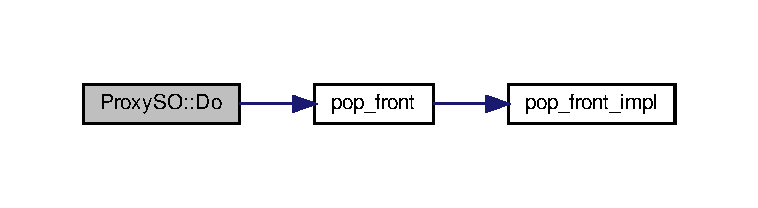
\includegraphics[width=350pt]{classProxySO_aea9532d196e05f80b2dd0de425df711f_cgraph}
\end{center}
\end{figure}
\mbox{\Hypertarget{classProxySO_affdd32b972bf9459a0f7ba37ec44a66a}\label{classProxySO_affdd32b972bf9459a0f7ba37ec44a66a}} 
\index{Proxy\+SO@{Proxy\+SO}!if@{if}}
\index{if@{if}!Proxy\+SO@{Proxy\+SO}}
\subsubsection{\texorpdfstring{if()}{if()}}
{\footnotesize\ttfamily template$<$typename R\+EQ , std\+::size\+\_\+t SZ$>$ \\
\hyperlink{classProxySO}{Proxy\+SO}$<$ R\+EQ, SZ $>$\+::if (\begin{DoxyParamCaption}\item[{!}]{handle\+\_\+ }\end{DoxyParamCaption})\hspace{0.3cm}{\ttfamily [inline]}}

\mbox{\Hypertarget{classProxySO_a1b036308a00c892930eb4e4955ed4716}\label{classProxySO_a1b036308a00c892930eb4e4955ed4716}} 
\index{Proxy\+SO@{Proxy\+SO}!Start\+Service\+Loop\+For\+Child@{Start\+Service\+Loop\+For\+Child}}
\index{Start\+Service\+Loop\+For\+Child@{Start\+Service\+Loop\+For\+Child}!Proxy\+SO@{Proxy\+SO}}
\subsubsection{\texorpdfstring{Start\+Service\+Loop\+For\+Child()}{StartServiceLoopForChild()}}
{\footnotesize\ttfamily template$<$typename R\+EQ , std\+::size\+\_\+t SZ$>$ \\
this \hyperlink{classProxySO}{Proxy\+SO}$<$ R\+EQ, SZ $>$\+::Start\+Service\+Loop\+For\+Child (\begin{DoxyParamCaption}{ }\end{DoxyParamCaption})}



\subsection{Member Data Documentation}
\mbox{\Hypertarget{classProxySO_a8db0f87ceb9dc54bd30b212394a74d09}\label{classProxySO_a8db0f87ceb9dc54bd30b212394a74d09}} 
\index{Proxy\+SO@{Proxy\+SO}!handle\+\_\+@{handle\+\_\+}}
\index{handle\+\_\+@{handle\+\_\+}!Proxy\+SO@{Proxy\+SO}}
\subsubsection{\texorpdfstring{handle\+\_\+}{handle\_}}
{\footnotesize\ttfamily template$<$typename R\+EQ , std\+::size\+\_\+t SZ$>$ \\
void$\ast$ \hyperlink{classProxySO}{Proxy\+SO}$<$ R\+EQ, SZ $>$\+::handle\+\_\+\hspace{0.3cm}{\ttfamily [private]}}



The documentation for this class was generated from the following file\+:\begin{DoxyCompactItemize}
\item 
include/\hyperlink{proxy_8hpp}{proxy.\+hpp}\end{DoxyCompactItemize}

\hypertarget{classSegment}{}\section{Segment$<$ SZ $>$ Class Template Reference}
\label{classSegment}\index{Segment$<$ S\+Z $>$@{Segment$<$ S\+Z $>$}}


{\ttfamily \#include $<$proxy.\+hpp$>$}



Collaboration diagram for Segment$<$ SZ $>$\+:
\nopagebreak
\begin{figure}[H]
\begin{center}
\leavevmode
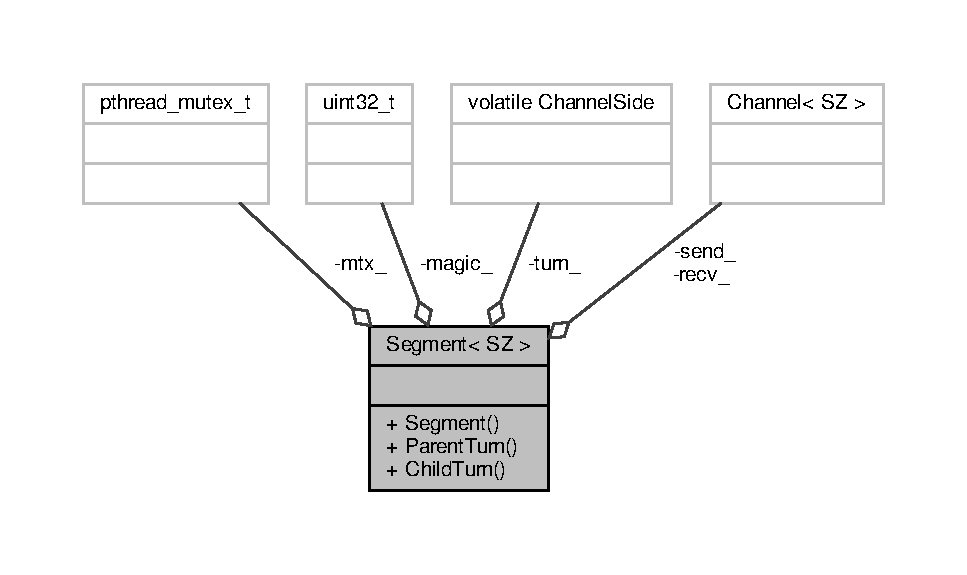
\includegraphics[width=350pt]{classSegment__coll__graph}
\end{center}
\end{figure}
\subsection*{Public Member Functions}
\begin{DoxyCompactItemize}
\item 
\hyperlink{classSegment_a9712a89eb6463d5ee551c2f60e30bd96}{Segment} ()
\item 
\+\_\+\+\_\+always\+\_\+inline bool \hyperlink{classSegment_a938f93ce0080d9c1b6098e38723aa52f}{Parent\+Turn} ()
\item 
\+\_\+\+\_\+always\+\_\+inline bool \hyperlink{classSegment_a502076154e0aaf26e1c67d8b37397b83}{Child\+Turn} ()
\end{DoxyCompactItemize}
\subsection*{Private Attributes}
\begin{DoxyCompactItemize}
\item 
volatile \hyperlink{proxy_8hpp_a249fda9ad200a554304ecf8de90d6877}{Channel\+Side} \hyperlink{classSegment_aa621c3ec3839a512ed61dd46406898de}{turn\+\_\+}
\item 
pthread\+\_\+mutex\+\_\+t \hyperlink{classSegment_af3cecd4372c6d3dc9aa482fa2da400e3}{mtx\+\_\+}
\item 
\hyperlink{classChannel}{Channel}$<$ SZ $>$ \hyperlink{classSegment_a237c718cfb7a495768efce6ca0c85c4c}{send\+\_\+}
\item 
\hyperlink{classChannel}{Channel}$<$ SZ $>$ \hyperlink{classSegment_a9fee642411f628501a3b0a972120c282}{recv\+\_\+}
\item 
uint32\+\_\+t \hyperlink{classSegment_abbfd0d6f6001b589b8dbc1e9ab837471}{magic\+\_\+} = \hyperlink{proxy_8hpp_af735db148c9e9f49d4feb7a4f5271b7a}{k\+Segment\+Magic}
\end{DoxyCompactItemize}
\subsection*{Friends}
\begin{DoxyCompactItemize}
\item 
class \hyperlink{classSegment_aa9880fe41382d4118e3f013f9058746d}{Segment\+Descriptor$<$ S\+Z $>$}
\end{DoxyCompactItemize}


\subsection{Constructor \& Destructor Documentation}
\mbox{\Hypertarget{classSegment_a9712a89eb6463d5ee551c2f60e30bd96}\label{classSegment_a9712a89eb6463d5ee551c2f60e30bd96}} 
\index{Segment@{Segment}!Segment@{Segment}}
\index{Segment@{Segment}!Segment@{Segment}}
\subsubsection{\texorpdfstring{Segment()}{Segment()}}
{\footnotesize\ttfamily template$<$std\+::size\+\_\+t SZ$>$ \\
\hyperlink{classSegment}{Segment}$<$ SZ $>$\+::\hyperlink{classSegment}{Segment} (\begin{DoxyParamCaption}{ }\end{DoxyParamCaption})\hspace{0.3cm}{\ttfamily [inline]}}



\subsection{Member Function Documentation}
\mbox{\Hypertarget{classSegment_a502076154e0aaf26e1c67d8b37397b83}\label{classSegment_a502076154e0aaf26e1c67d8b37397b83}} 
\index{Segment@{Segment}!Child\+Turn@{Child\+Turn}}
\index{Child\+Turn@{Child\+Turn}!Segment@{Segment}}
\subsubsection{\texorpdfstring{Child\+Turn()}{ChildTurn()}}
{\footnotesize\ttfamily template$<$std\+::size\+\_\+t SZ$>$ \\
\+\_\+\+\_\+always\+\_\+inline bool \hyperlink{classSegment}{Segment}$<$ SZ $>$\+::Child\+Turn (\begin{DoxyParamCaption}{ }\end{DoxyParamCaption})\hspace{0.3cm}{\ttfamily [inline]}}

\mbox{\Hypertarget{classSegment_a938f93ce0080d9c1b6098e38723aa52f}\label{classSegment_a938f93ce0080d9c1b6098e38723aa52f}} 
\index{Segment@{Segment}!Parent\+Turn@{Parent\+Turn}}
\index{Parent\+Turn@{Parent\+Turn}!Segment@{Segment}}
\subsubsection{\texorpdfstring{Parent\+Turn()}{ParentTurn()}}
{\footnotesize\ttfamily template$<$std\+::size\+\_\+t SZ$>$ \\
\+\_\+\+\_\+always\+\_\+inline bool \hyperlink{classSegment}{Segment}$<$ SZ $>$\+::Parent\+Turn (\begin{DoxyParamCaption}{ }\end{DoxyParamCaption})\hspace{0.3cm}{\ttfamily [inline]}}



\subsection{Friends And Related Function Documentation}
\mbox{\Hypertarget{classSegment_aa9880fe41382d4118e3f013f9058746d}\label{classSegment_aa9880fe41382d4118e3f013f9058746d}} 
\index{Segment@{Segment}!Segment\+Descriptor$<$ S\+Z $>$@{Segment\+Descriptor$<$ S\+Z $>$}}
\index{Segment\+Descriptor$<$ S\+Z $>$@{Segment\+Descriptor$<$ S\+Z $>$}!Segment@{Segment}}
\subsubsection{\texorpdfstring{Segment\+Descriptor$<$ S\+Z $>$}{SegmentDescriptor< SZ >}}
{\footnotesize\ttfamily template$<$std\+::size\+\_\+t SZ$>$ \\
friend class \hyperlink{classSegmentDescriptor}{Segment\+Descriptor}$<$ SZ $>$\hspace{0.3cm}{\ttfamily [friend]}}



\subsection{Member Data Documentation}
\mbox{\Hypertarget{classSegment_abbfd0d6f6001b589b8dbc1e9ab837471}\label{classSegment_abbfd0d6f6001b589b8dbc1e9ab837471}} 
\index{Segment@{Segment}!magic\+\_\+@{magic\+\_\+}}
\index{magic\+\_\+@{magic\+\_\+}!Segment@{Segment}}
\subsubsection{\texorpdfstring{magic\+\_\+}{magic\_}}
{\footnotesize\ttfamily template$<$std\+::size\+\_\+t SZ$>$ \\
uint32\+\_\+t \hyperlink{classSegment}{Segment}$<$ SZ $>$\+::magic\+\_\+ = \hyperlink{proxy_8hpp_af735db148c9e9f49d4feb7a4f5271b7a}{k\+Segment\+Magic}\hspace{0.3cm}{\ttfamily [private]}}

\mbox{\Hypertarget{classSegment_af3cecd4372c6d3dc9aa482fa2da400e3}\label{classSegment_af3cecd4372c6d3dc9aa482fa2da400e3}} 
\index{Segment@{Segment}!mtx\+\_\+@{mtx\+\_\+}}
\index{mtx\+\_\+@{mtx\+\_\+}!Segment@{Segment}}
\subsubsection{\texorpdfstring{mtx\+\_\+}{mtx\_}}
{\footnotesize\ttfamily template$<$std\+::size\+\_\+t SZ$>$ \\
pthread\+\_\+mutex\+\_\+t \hyperlink{classSegment}{Segment}$<$ SZ $>$\+::mtx\+\_\+\hspace{0.3cm}{\ttfamily [private]}}

\mbox{\Hypertarget{classSegment_a9fee642411f628501a3b0a972120c282}\label{classSegment_a9fee642411f628501a3b0a972120c282}} 
\index{Segment@{Segment}!recv\+\_\+@{recv\+\_\+}}
\index{recv\+\_\+@{recv\+\_\+}!Segment@{Segment}}
\subsubsection{\texorpdfstring{recv\+\_\+}{recv\_}}
{\footnotesize\ttfamily template$<$std\+::size\+\_\+t SZ$>$ \\
\hyperlink{classChannel}{Channel}$<$SZ$>$ \hyperlink{classSegment}{Segment}$<$ SZ $>$\+::recv\+\_\+\hspace{0.3cm}{\ttfamily [private]}}

\mbox{\Hypertarget{classSegment_a237c718cfb7a495768efce6ca0c85c4c}\label{classSegment_a237c718cfb7a495768efce6ca0c85c4c}} 
\index{Segment@{Segment}!send\+\_\+@{send\+\_\+}}
\index{send\+\_\+@{send\+\_\+}!Segment@{Segment}}
\subsubsection{\texorpdfstring{send\+\_\+}{send\_}}
{\footnotesize\ttfamily template$<$std\+::size\+\_\+t SZ$>$ \\
\hyperlink{classChannel}{Channel}$<$SZ$>$ \hyperlink{classSegment}{Segment}$<$ SZ $>$\+::send\+\_\+\hspace{0.3cm}{\ttfamily [private]}}

\mbox{\Hypertarget{classSegment_aa621c3ec3839a512ed61dd46406898de}\label{classSegment_aa621c3ec3839a512ed61dd46406898de}} 
\index{Segment@{Segment}!turn\+\_\+@{turn\+\_\+}}
\index{turn\+\_\+@{turn\+\_\+}!Segment@{Segment}}
\subsubsection{\texorpdfstring{turn\+\_\+}{turn\_}}
{\footnotesize\ttfamily template$<$std\+::size\+\_\+t SZ$>$ \\
volatile \hyperlink{proxy_8hpp_a249fda9ad200a554304ecf8de90d6877}{Channel\+Side} \hyperlink{classSegment}{Segment}$<$ SZ $>$\+::turn\+\_\+\hspace{0.3cm}{\ttfamily [private]}}



The documentation for this class was generated from the following file\+:\begin{DoxyCompactItemize}
\item 
include/\hyperlink{proxy_8hpp}{proxy.\+hpp}\end{DoxyCompactItemize}

\hypertarget{classSegmentDescriptor}{}\section{Segment\+Descriptor$<$ SZ $>$ Class Template Reference}
\label{classSegmentDescriptor}\index{Segment\+Descriptor$<$ S\+Z $>$@{Segment\+Descriptor$<$ S\+Z $>$}}


{\ttfamily \#include $<$proxy.\+hpp$>$}



Collaboration diagram for Segment\+Descriptor$<$ SZ $>$\+:
\nopagebreak
\begin{figure}[H]
\begin{center}
\leavevmode
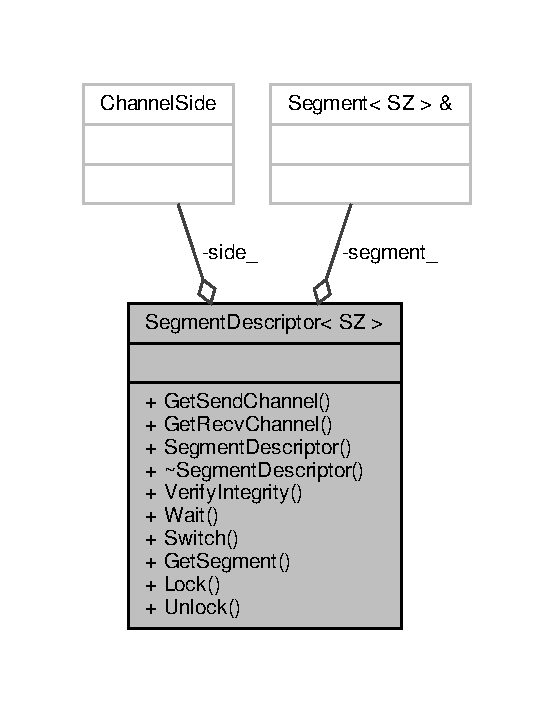
\includegraphics[width=266pt]{classSegmentDescriptor__coll__graph}
\end{center}
\end{figure}
\subsection*{Public Member Functions}
\begin{DoxyCompactItemize}
\item 
\hyperlink{classChannel}{Channel}$<$ SZ $>$ \& \hyperlink{classSegmentDescriptor_a2f9e15ad56caf25a73a76ebb9dcfd26e}{Get\+Send\+Channel} () const
\item 
\hyperlink{classChannel}{Channel}$<$ SZ $>$ \& \hyperlink{classSegmentDescriptor_a3b7cb0548fb39870191fce0d42b20494}{Get\+Recv\+Channel} () const
\item 
\hyperlink{classSegmentDescriptor_a042a4c43ff3213dc643a3b8fb40c9b05}{Segment\+Descriptor} (\hyperlink{proxy_8hpp_a249fda9ad200a554304ecf8de90d6877}{Channel\+Side} side, \hyperlink{classSegment}{Segment}$<$ SZ $>$ \&seg)
\item 
\hyperlink{classSegmentDescriptor_a1b8897effdc10f093db07328aa9eb64f}{$\sim$\+Segment\+Descriptor} ()
\item 
bool \hyperlink{classSegmentDescriptor_a2dd29d04ba59a348aa2188f86a5c3cff}{Verify\+Integrity} () const
\item 
void \hyperlink{classSegmentDescriptor_a253f68680c02ea71b6504f5ce9dba741}{Wait} ()
\item 
void \hyperlink{classSegmentDescriptor_aca5320d3edfabec89285c251b8c25094}{Switch} ()
\item 
\hyperlink{classSegment}{Segment}$<$ SZ $>$ \& \hyperlink{classSegmentDescriptor_a11f3ac05bd4f223fac0c67e54b44cd7f}{Get\+Segment} () const
\end{DoxyCompactItemize}
\subsection*{Static Public Member Functions}
\begin{DoxyCompactItemize}
\item 
static \+\_\+\+\_\+always\+\_\+inline void \hyperlink{classSegmentDescriptor_ab5cc70efd5c89b3466174bb48e951ede}{Lock} (pthread\+\_\+mutex\+\_\+t \&mtx)
\item 
static \+\_\+\+\_\+always\+\_\+inline void \hyperlink{classSegmentDescriptor_aed5e493d85b1132056e180861799557d}{Unlock} (pthread\+\_\+mutex\+\_\+t \&mtx)
\end{DoxyCompactItemize}
\subsection*{Private Attributes}
\begin{DoxyCompactItemize}
\item 
\hyperlink{proxy_8hpp_a249fda9ad200a554304ecf8de90d6877}{Channel\+Side} \hyperlink{classSegmentDescriptor_a0e3fbc1517507dd8ce948232cfd5508b}{side\+\_\+}
\item 
\hyperlink{classSegment}{Segment}$<$ SZ $>$ \& \hyperlink{classSegmentDescriptor_ad0c2fdf75d6c44f0b01e3e8f7a7a5977}{segment\+\_\+}
\end{DoxyCompactItemize}


\subsection{Constructor \& Destructor Documentation}
\mbox{\Hypertarget{classSegmentDescriptor_a042a4c43ff3213dc643a3b8fb40c9b05}\label{classSegmentDescriptor_a042a4c43ff3213dc643a3b8fb40c9b05}} 
\index{Segment\+Descriptor@{Segment\+Descriptor}!Segment\+Descriptor@{Segment\+Descriptor}}
\index{Segment\+Descriptor@{Segment\+Descriptor}!Segment\+Descriptor@{Segment\+Descriptor}}
\subsubsection{\texorpdfstring{Segment\+Descriptor()}{SegmentDescriptor()}}
{\footnotesize\ttfamily template$<$std\+::size\+\_\+t SZ$>$ \\
\hyperlink{classSegmentDescriptor}{Segment\+Descriptor}$<$ SZ $>$\+::\hyperlink{classSegmentDescriptor}{Segment\+Descriptor} (\begin{DoxyParamCaption}\item[{\hyperlink{proxy_8hpp_a249fda9ad200a554304ecf8de90d6877}{Channel\+Side}}]{side,  }\item[{\hyperlink{classSegment}{Segment}$<$ SZ $>$ \&}]{seg }\end{DoxyParamCaption})\hspace{0.3cm}{\ttfamily [inline]}}

\mbox{\Hypertarget{classSegmentDescriptor_a1b8897effdc10f093db07328aa9eb64f}\label{classSegmentDescriptor_a1b8897effdc10f093db07328aa9eb64f}} 
\index{Segment\+Descriptor@{Segment\+Descriptor}!````~Segment\+Descriptor@{$\sim$\+Segment\+Descriptor}}
\index{````~Segment\+Descriptor@{$\sim$\+Segment\+Descriptor}!Segment\+Descriptor@{Segment\+Descriptor}}
\subsubsection{\texorpdfstring{$\sim$\+Segment\+Descriptor()}{~SegmentDescriptor()}}
{\footnotesize\ttfamily template$<$std\+::size\+\_\+t SZ$>$ \\
\hyperlink{classSegmentDescriptor}{Segment\+Descriptor}$<$ SZ $>$\+::$\sim$\hyperlink{classSegmentDescriptor}{Segment\+Descriptor} (\begin{DoxyParamCaption}{ }\end{DoxyParamCaption})\hspace{0.3cm}{\ttfamily [inline]}}



\subsection{Member Function Documentation}
\mbox{\Hypertarget{classSegmentDescriptor_a3b7cb0548fb39870191fce0d42b20494}\label{classSegmentDescriptor_a3b7cb0548fb39870191fce0d42b20494}} 
\index{Segment\+Descriptor@{Segment\+Descriptor}!Get\+Recv\+Channel@{Get\+Recv\+Channel}}
\index{Get\+Recv\+Channel@{Get\+Recv\+Channel}!Segment\+Descriptor@{Segment\+Descriptor}}
\subsubsection{\texorpdfstring{Get\+Recv\+Channel()}{GetRecvChannel()}}
{\footnotesize\ttfamily template$<$std\+::size\+\_\+t SZ$>$ \\
\hyperlink{classChannel}{Channel}$<$SZ$>$\& \hyperlink{classSegmentDescriptor}{Segment\+Descriptor}$<$ SZ $>$\+::Get\+Recv\+Channel (\begin{DoxyParamCaption}{ }\end{DoxyParamCaption}) const\hspace{0.3cm}{\ttfamily [inline]}}

\mbox{\Hypertarget{classSegmentDescriptor_a11f3ac05bd4f223fac0c67e54b44cd7f}\label{classSegmentDescriptor_a11f3ac05bd4f223fac0c67e54b44cd7f}} 
\index{Segment\+Descriptor@{Segment\+Descriptor}!Get\+Segment@{Get\+Segment}}
\index{Get\+Segment@{Get\+Segment}!Segment\+Descriptor@{Segment\+Descriptor}}
\subsubsection{\texorpdfstring{Get\+Segment()}{GetSegment()}}
{\footnotesize\ttfamily template$<$std\+::size\+\_\+t SZ$>$ \\
\hyperlink{classSegment}{Segment}$<$SZ$>$\& \hyperlink{classSegmentDescriptor}{Segment\+Descriptor}$<$ SZ $>$\+::Get\+Segment (\begin{DoxyParamCaption}{ }\end{DoxyParamCaption}) const\hspace{0.3cm}{\ttfamily [inline]}}

\mbox{\Hypertarget{classSegmentDescriptor_a2f9e15ad56caf25a73a76ebb9dcfd26e}\label{classSegmentDescriptor_a2f9e15ad56caf25a73a76ebb9dcfd26e}} 
\index{Segment\+Descriptor@{Segment\+Descriptor}!Get\+Send\+Channel@{Get\+Send\+Channel}}
\index{Get\+Send\+Channel@{Get\+Send\+Channel}!Segment\+Descriptor@{Segment\+Descriptor}}
\subsubsection{\texorpdfstring{Get\+Send\+Channel()}{GetSendChannel()}}
{\footnotesize\ttfamily template$<$std\+::size\+\_\+t SZ$>$ \\
\hyperlink{classChannel}{Channel}$<$SZ$>$\& \hyperlink{classSegmentDescriptor}{Segment\+Descriptor}$<$ SZ $>$\+::Get\+Send\+Channel (\begin{DoxyParamCaption}{ }\end{DoxyParamCaption}) const\hspace{0.3cm}{\ttfamily [inline]}}

\mbox{\Hypertarget{classSegmentDescriptor_ab5cc70efd5c89b3466174bb48e951ede}\label{classSegmentDescriptor_ab5cc70efd5c89b3466174bb48e951ede}} 
\index{Segment\+Descriptor@{Segment\+Descriptor}!Lock@{Lock}}
\index{Lock@{Lock}!Segment\+Descriptor@{Segment\+Descriptor}}
\subsubsection{\texorpdfstring{Lock()}{Lock()}}
{\footnotesize\ttfamily template$<$std\+::size\+\_\+t SZ$>$ \\
static \+\_\+\+\_\+always\+\_\+inline void \hyperlink{classSegmentDescriptor}{Segment\+Descriptor}$<$ SZ $>$\+::Lock (\begin{DoxyParamCaption}\item[{pthread\+\_\+mutex\+\_\+t \&}]{mtx }\end{DoxyParamCaption})\hspace{0.3cm}{\ttfamily [inline]}, {\ttfamily [static]}}

Another process has dies while holding this mutex. We should clean up after that process, and unlock them mutex when we are done with it.

Tell the runtime that we have taken care of the situation.\mbox{\Hypertarget{classSegmentDescriptor_aca5320d3edfabec89285c251b8c25094}\label{classSegmentDescriptor_aca5320d3edfabec89285c251b8c25094}} 
\index{Segment\+Descriptor@{Segment\+Descriptor}!Switch@{Switch}}
\index{Switch@{Switch}!Segment\+Descriptor@{Segment\+Descriptor}}
\subsubsection{\texorpdfstring{Switch()}{Switch()}}
{\footnotesize\ttfamily template$<$std\+::size\+\_\+t SZ$>$ \\
void \hyperlink{classSegmentDescriptor}{Segment\+Descriptor}$<$ SZ $>$\+::Switch (\begin{DoxyParamCaption}{ }\end{DoxyParamCaption})\hspace{0.3cm}{\ttfamily [inline]}}

\mbox{\Hypertarget{classSegmentDescriptor_aed5e493d85b1132056e180861799557d}\label{classSegmentDescriptor_aed5e493d85b1132056e180861799557d}} 
\index{Segment\+Descriptor@{Segment\+Descriptor}!Unlock@{Unlock}}
\index{Unlock@{Unlock}!Segment\+Descriptor@{Segment\+Descriptor}}
\subsubsection{\texorpdfstring{Unlock()}{Unlock()}}
{\footnotesize\ttfamily template$<$std\+::size\+\_\+t SZ$>$ \\
static \+\_\+\+\_\+always\+\_\+inline void \hyperlink{classSegmentDescriptor}{Segment\+Descriptor}$<$ SZ $>$\+::Unlock (\begin{DoxyParamCaption}\item[{pthread\+\_\+mutex\+\_\+t \&}]{mtx }\end{DoxyParamCaption})\hspace{0.3cm}{\ttfamily [inline]}, {\ttfamily [static]}}

\mbox{\Hypertarget{classSegmentDescriptor_a2dd29d04ba59a348aa2188f86a5c3cff}\label{classSegmentDescriptor_a2dd29d04ba59a348aa2188f86a5c3cff}} 
\index{Segment\+Descriptor@{Segment\+Descriptor}!Verify\+Integrity@{Verify\+Integrity}}
\index{Verify\+Integrity@{Verify\+Integrity}!Segment\+Descriptor@{Segment\+Descriptor}}
\subsubsection{\texorpdfstring{Verify\+Integrity()}{VerifyIntegrity()}}
{\footnotesize\ttfamily template$<$std\+::size\+\_\+t SZ$>$ \\
bool \hyperlink{classSegmentDescriptor}{Segment\+Descriptor}$<$ SZ $>$\+::Verify\+Integrity (\begin{DoxyParamCaption}{ }\end{DoxyParamCaption}) const\hspace{0.3cm}{\ttfamily [inline]}}

\mbox{\Hypertarget{classSegmentDescriptor_a253f68680c02ea71b6504f5ce9dba741}\label{classSegmentDescriptor_a253f68680c02ea71b6504f5ce9dba741}} 
\index{Segment\+Descriptor@{Segment\+Descriptor}!Wait@{Wait}}
\index{Wait@{Wait}!Segment\+Descriptor@{Segment\+Descriptor}}
\subsubsection{\texorpdfstring{Wait()}{Wait()}}
{\footnotesize\ttfamily template$<$std\+::size\+\_\+t SZ$>$ \\
void \hyperlink{classSegmentDescriptor}{Segment\+Descriptor}$<$ SZ $>$\+::Wait (\begin{DoxyParamCaption}{ }\end{DoxyParamCaption})\hspace{0.3cm}{\ttfamily [inline]}}



\subsection{Member Data Documentation}
\mbox{\Hypertarget{classSegmentDescriptor_ad0c2fdf75d6c44f0b01e3e8f7a7a5977}\label{classSegmentDescriptor_ad0c2fdf75d6c44f0b01e3e8f7a7a5977}} 
\index{Segment\+Descriptor@{Segment\+Descriptor}!segment\+\_\+@{segment\+\_\+}}
\index{segment\+\_\+@{segment\+\_\+}!Segment\+Descriptor@{Segment\+Descriptor}}
\subsubsection{\texorpdfstring{segment\+\_\+}{segment\_}}
{\footnotesize\ttfamily template$<$std\+::size\+\_\+t SZ$>$ \\
\hyperlink{classSegment}{Segment}$<$SZ$>$\& \hyperlink{classSegmentDescriptor}{Segment\+Descriptor}$<$ SZ $>$\+::segment\+\_\+\hspace{0.3cm}{\ttfamily [private]}}

\mbox{\Hypertarget{classSegmentDescriptor_a0e3fbc1517507dd8ce948232cfd5508b}\label{classSegmentDescriptor_a0e3fbc1517507dd8ce948232cfd5508b}} 
\index{Segment\+Descriptor@{Segment\+Descriptor}!side\+\_\+@{side\+\_\+}}
\index{side\+\_\+@{side\+\_\+}!Segment\+Descriptor@{Segment\+Descriptor}}
\subsubsection{\texorpdfstring{side\+\_\+}{side\_}}
{\footnotesize\ttfamily template$<$std\+::size\+\_\+t SZ$>$ \\
\hyperlink{proxy_8hpp_a249fda9ad200a554304ecf8de90d6877}{Channel\+Side} \hyperlink{classSegmentDescriptor}{Segment\+Descriptor}$<$ SZ $>$\+::side\+\_\+\hspace{0.3cm}{\ttfamily [private]}}



The documentation for this class was generated from the following file\+:\begin{DoxyCompactItemize}
\item 
include/\hyperlink{proxy_8hpp}{proxy.\+hpp}\end{DoxyCompactItemize}

\hypertarget{classStub}{}\section{Stub$<$ SZ $>$ Class Template Reference}
\label{classStub}\index{Stub$<$ S\+Z $>$@{Stub$<$ S\+Z $>$}}


{\ttfamily \#include $<$proxy.\+hpp$>$}



Collaboration diagram for Stub$<$ SZ $>$\+:
\nopagebreak
\begin{figure}[H]
\begin{center}
\leavevmode
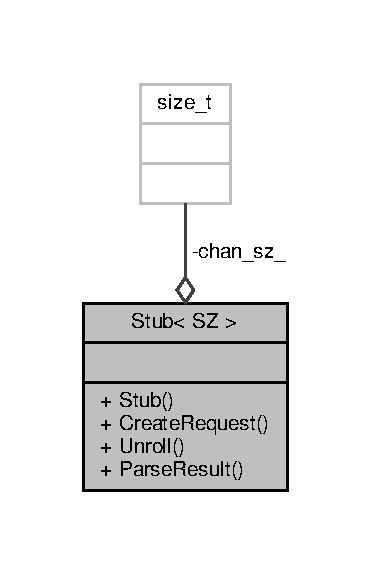
\includegraphics[width=178pt]{classStub__coll__graph}
\end{center}
\end{figure}
\subsection*{Public Member Functions}
\begin{DoxyCompactItemize}
\item 
\hyperlink{classStub_ae7629b6acb5ded1513e9ab73f293f93e}{Stub} ()
\item 
{\footnotesize template$<$typename... Args$>$ }\\void \hyperlink{classStub_ab83bdd8197df762e5763c2ef937ae0e5}{Create\+Request} (void $\ast$base, Args... args)
\item 
{\footnotesize template$<$typename T , typename... Args$>$ }\\void \hyperlink{classStub_aeaed7e40c227acf10dd0b82a8a5d0306}{Unroll} (void $\ast$base, T t, Args... args)
\item 
{\footnotesize template$<$typename R $>$ }\\R \hyperlink{classStub_a3eb7ab0bf78f5a7bb7668bc70e9dfc88}{Parse\+Result} (void $\ast$base)
\end{DoxyCompactItemize}
\subsection*{Private Attributes}
\begin{DoxyCompactItemize}
\item 
std\+::size\+\_\+t \hyperlink{classStub_a758cf7539d362589c476e72ed8cb01cf}{chan\+\_\+sz\+\_\+}
\end{DoxyCompactItemize}


\subsection{Constructor \& Destructor Documentation}
\mbox{\Hypertarget{classStub_ae7629b6acb5ded1513e9ab73f293f93e}\label{classStub_ae7629b6acb5ded1513e9ab73f293f93e}} 
\index{Stub@{Stub}!Stub@{Stub}}
\index{Stub@{Stub}!Stub@{Stub}}
\subsubsection{\texorpdfstring{Stub()}{Stub()}}
{\footnotesize\ttfamily template$<$std\+::size\+\_\+t SZ$>$ \\
\hyperlink{classStub}{Stub}$<$ SZ $>$\+::\hyperlink{classStub}{Stub} (\begin{DoxyParamCaption}{ }\end{DoxyParamCaption})\hspace{0.3cm}{\ttfamily [inline]}}



\subsection{Member Function Documentation}
\mbox{\Hypertarget{classStub_ab83bdd8197df762e5763c2ef937ae0e5}\label{classStub_ab83bdd8197df762e5763c2ef937ae0e5}} 
\index{Stub@{Stub}!Create\+Request@{Create\+Request}}
\index{Create\+Request@{Create\+Request}!Stub@{Stub}}
\subsubsection{\texorpdfstring{Create\+Request()}{CreateRequest()}}
{\footnotesize\ttfamily template$<$std\+::size\+\_\+t SZ$>$ \\
template$<$typename... Args$>$ \\
void \hyperlink{classStub}{Stub}$<$ SZ $>$\+::Create\+Request (\begin{DoxyParamCaption}\item[{void $\ast$}]{base,  }\item[{Args...}]{args }\end{DoxyParamCaption})\hspace{0.3cm}{\ttfamily [inline]}}

\mbox{\Hypertarget{classStub_a3eb7ab0bf78f5a7bb7668bc70e9dfc88}\label{classStub_a3eb7ab0bf78f5a7bb7668bc70e9dfc88}} 
\index{Stub@{Stub}!Parse\+Result@{Parse\+Result}}
\index{Parse\+Result@{Parse\+Result}!Stub@{Stub}}
\subsubsection{\texorpdfstring{Parse\+Result()}{ParseResult()}}
{\footnotesize\ttfamily template$<$std\+::size\+\_\+t SZ$>$ \\
template$<$typename R $>$ \\
R \hyperlink{classStub}{Stub}$<$ SZ $>$\+::Parse\+Result (\begin{DoxyParamCaption}\item[{void $\ast$}]{base }\end{DoxyParamCaption})\hspace{0.3cm}{\ttfamily [inline]}}

\mbox{\Hypertarget{classStub_aeaed7e40c227acf10dd0b82a8a5d0306}\label{classStub_aeaed7e40c227acf10dd0b82a8a5d0306}} 
\index{Stub@{Stub}!Unroll@{Unroll}}
\index{Unroll@{Unroll}!Stub@{Stub}}
\subsubsection{\texorpdfstring{Unroll()}{Unroll()}}
{\footnotesize\ttfamily template$<$std\+::size\+\_\+t SZ$>$ \\
template$<$typename T , typename... Args$>$ \\
void \hyperlink{classStub}{Stub}$<$ SZ $>$\+::Unroll (\begin{DoxyParamCaption}\item[{void $\ast$}]{base,  }\item[{T}]{t,  }\item[{Args...}]{args }\end{DoxyParamCaption})\hspace{0.3cm}{\ttfamily [inline]}}



\subsection{Member Data Documentation}
\mbox{\Hypertarget{classStub_a758cf7539d362589c476e72ed8cb01cf}\label{classStub_a758cf7539d362589c476e72ed8cb01cf}} 
\index{Stub@{Stub}!chan\+\_\+sz\+\_\+@{chan\+\_\+sz\+\_\+}}
\index{chan\+\_\+sz\+\_\+@{chan\+\_\+sz\+\_\+}!Stub@{Stub}}
\subsubsection{\texorpdfstring{chan\+\_\+sz\+\_\+}{chan\_sz\_}}
{\footnotesize\ttfamily template$<$std\+::size\+\_\+t SZ$>$ \\
std\+::size\+\_\+t \hyperlink{classStub}{Stub}$<$ SZ $>$\+::chan\+\_\+sz\+\_\+\hspace{0.3cm}{\ttfamily [private]}}



The documentation for this class was generated from the following file\+:\begin{DoxyCompactItemize}
\item 
include/\hyperlink{proxy_8hpp}{proxy.\+hpp}\end{DoxyCompactItemize}

\chapter{File Documentation}
\hypertarget{proxy_8hpp}{}\section{include/proxy.hpp File Reference}
\label{proxy_8hpp}\index{include/proxy.\+hpp@{include/proxy.\+hpp}}
{\ttfamily \#include $<$atomic$>$}\newline
{\ttfamily \#include $<$cstdint$>$}\newline
{\ttfamily \#include $<$iostream$>$}\newline
{\ttfamily \#include $<$memory$>$}\newline
{\ttfamily \#include $<$type\+\_\+traits$>$}\newline
{\ttfamily \#include $<$exception$>$}\newline
{\ttfamily \#include $<$functional$>$}\newline
{\ttfamily \#include $<$dlfcn.\+h$>$}\newline
{\ttfamily \#include $<$immintrin.\+h$>$}\newline
{\ttfamily \#include $<$sys/mman.\+h$>$}\newline
{\ttfamily \#include $<$pthread.\+h$>$}\newline
{\ttfamily \#include $<$unistd.\+h$>$}\newline
{\ttfamily \#include $<$errno.\+h$>$}\newline
{\ttfamily \#include $<$stdlib.\+h$>$}\newline
{\ttfamily \#include $<$string.\+h$>$}\newline
{\ttfamily \#include $<$signal.\+h$>$}\newline
Include dependency graph for proxy.\+hpp\+:
\nopagebreak
\begin{figure}[H]
\begin{center}
\leavevmode
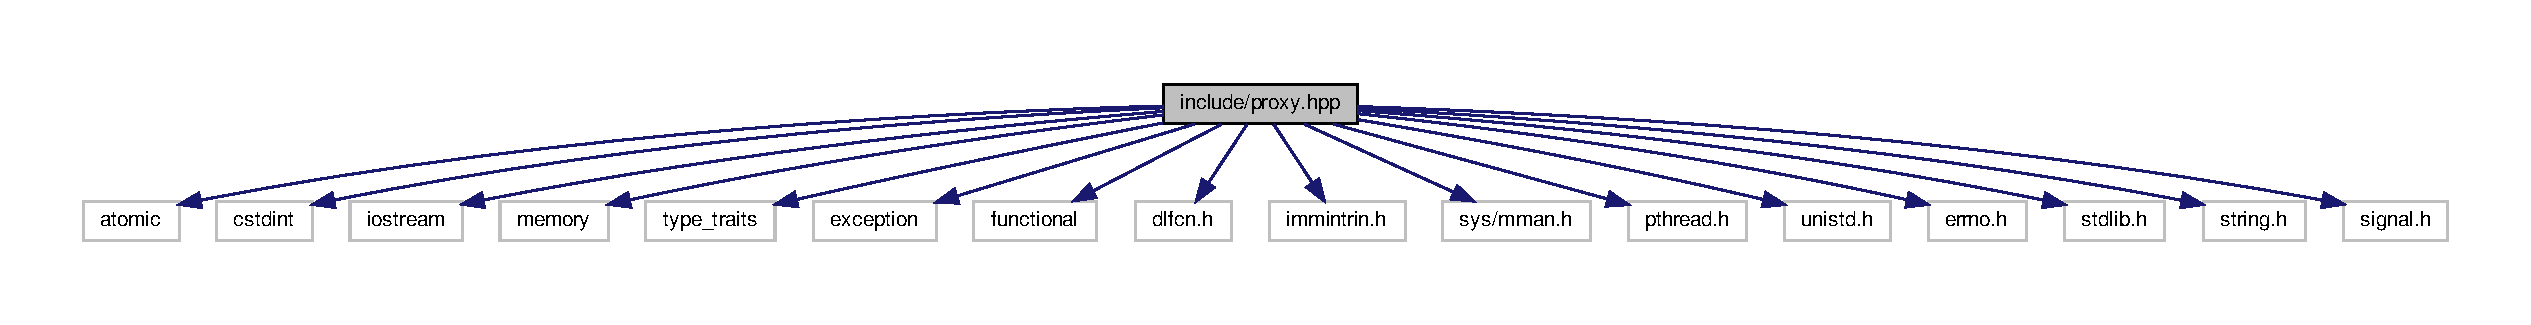
\includegraphics[width=350pt]{proxy_8hpp__incl}
\end{center}
\end{figure}
This graph shows which files directly or indirectly include this file\+:
\nopagebreak
\begin{figure}[H]
\begin{center}
\leavevmode
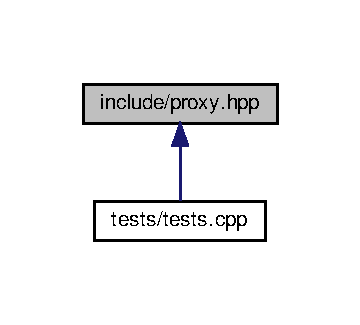
\includegraphics[width=173pt]{proxy_8hpp__dep__incl}
\end{center}
\end{figure}
\subsection*{Classes}
\begin{DoxyCompactItemize}
\item 
class \hyperlink{classParentTerminated}{Parent\+Terminated}
\item 
class \hyperlink{classChildTerminated}{Child\+Terminated}
\item 
class \hyperlink{classOperationFailed}{Operation\+Failed}
\item 
class \hyperlink{classSegmentDescriptor}{Segment\+Descriptor$<$ S\+Z $>$}
\item 
class \hyperlink{classChannel}{Channel$<$ S\+Z $>$}
\item 
class \hyperlink{classSegment}{Segment$<$ S\+Z $>$}
\item 
class \hyperlink{classSegmentDescriptor}{Segment\+Descriptor$<$ S\+Z $>$}
\item 
class \hyperlink{classStub}{Stub$<$ S\+Z $>$}
\item 
class \hyperlink{classBaseProxy}{Base\+Proxy}
\item 
class \hyperlink{classAbstractProxy}{Abstract\+Proxy$<$ R\+E\+Q, S\+Z $>$}
\item 
class \hyperlink{classProxyDirect}{Proxy\+Direct$<$ R\+E\+Q, S\+Z, S\+E\+R\+V $>$}
\item 
class \hyperlink{classProxySO}{Proxy\+S\+O$<$ R\+E\+Q, S\+Z $>$}
\item 
class \hyperlink{classProxy}{Proxy$<$ R\+E\+Q, S\+Z, S\+E\+R\+V $>$}
\end{DoxyCompactItemize}
\subsection*{Macros}
\begin{DoxyCompactItemize}
\item 
\#define \hyperlink{proxy_8hpp_a7d467c1d283fdfa1f2081ba1e0d01b6e}{P\+A\+G\+E\+\_\+\+S\+I\+ZE}~4096
\item 
\#define \hyperlink{proxy_8hpp_ab7ef411847b693e526afebd2891a96e5}{C\+H\+A\+N\+\_\+\+S\+I\+ZE}~4096
\item 
\#define \hyperlink{proxy_8hpp_ac97a6b877f67d3955003a0f410674d10}{P\+R\+O\+X\+Y\+\_\+\+L\+OG}(c)~std\+::cerr
\end{DoxyCompactItemize}
\subsection*{Enumerations}
\begin{DoxyCompactItemize}
\item 
enum \hyperlink{proxy_8hpp_afebd7ebbad7f3100ab6bf934c5782c35}{D\+C\+O\+DE} \{ \hyperlink{proxy_8hpp_afebd7ebbad7f3100ab6bf934c5782c35a7b9ac307be3862f601f7a65c1c69f4d1}{k\+D\+Code\+\_\+\+Init}, 
\hyperlink{proxy_8hpp_afebd7ebbad7f3100ab6bf934c5782c35a2f1ade63ec79f35261d2df70e2312681}{k\+D\+Code\+\_\+\+Limit}, 
\hyperlink{proxy_8hpp_afebd7ebbad7f3100ab6bf934c5782c35aeb7819c435f1fb1e6e7bc083a05a91d3}{k\+D\+Code\+\_\+\+Shutdown}, 
\hyperlink{proxy_8hpp_afebd7ebbad7f3100ab6bf934c5782c35aa8caee722ca6ce827ce021a9e82550f2}{k\+D\+Code\+\_\+\+Task}
 \}
\item 
enum \hyperlink{proxy_8hpp_abdf990fbe51b4c9d3fdcc2fc3c6f9219}{Channel\+Status} \{ \hyperlink{proxy_8hpp_abdf990fbe51b4c9d3fdcc2fc3c6f9219a7fb3bf49ba349ca1a266be41df447b5b}{k\+Open}, 
\hyperlink{proxy_8hpp_abdf990fbe51b4c9d3fdcc2fc3c6f9219a44be8f61450ed22be5adcc881a95570f}{k\+Closed}
 \}
\item 
enum \hyperlink{proxy_8hpp_a249fda9ad200a554304ecf8de90d6877}{Channel\+Side} \{ \hyperlink{proxy_8hpp_a249fda9ad200a554304ecf8de90d6877a9c4b0fadea329894df39608542f6d656}{k\+Parent}, 
\hyperlink{proxy_8hpp_a249fda9ad200a554304ecf8de90d6877a6ea35dfa8911c238573f5ca06db2e497}{k\+Child}
 \}
\end{DoxyCompactItemize}
\subsection*{Functions}
\begin{DoxyCompactItemize}
\item 
{\footnotesize template$<$typename Tuple , std\+::size\+\_\+t ... Is$>$ }\\auto \hyperlink{proxy_8hpp_ae5e7ef9b08c7340386e7eccab535c7f0}{pop\+\_\+front\+\_\+impl} (const Tuple \&tuple, std\+::index\+\_\+sequence$<$ Is... $>$)
\item 
{\footnotesize template$<$typename Tuple $>$ }\\auto \hyperlink{proxy_8hpp_a6ba8a69fe5dfb69975740463e80ce89b}{pop\+\_\+front} (const Tuple \&tuple)
\item 
void \hyperlink{proxy_8hpp_a4f31a6fd48ee5d4579ae4aaaa3cae285}{sig\+\_\+handler} (int signo)
\end{DoxyCompactItemize}
\subsection*{Variables}
\begin{DoxyCompactItemize}
\item 
constexpr int \hyperlink{proxy_8hpp_a8b43c81ee7b8a4288c1cc31aad967e7d}{k\+S\+H\+M\+Alignment} = 8
\item 
bool \hyperlink{proxy_8hpp_afc2f556ffb367cbd8559aa26d9baa913}{parent\+\_\+terminated} = false
\item 
bool \hyperlink{proxy_8hpp_a0fa3e25df0e6e54f52f9aea616c50d3b}{child\+\_\+terminated} = false
\item 
constexpr uint32\+\_\+t \hyperlink{proxy_8hpp_af735db148c9e9f49d4feb7a4f5271b7a}{k\+Segment\+Magic} = 0xc7390fbc
\end{DoxyCompactItemize}


\subsection{Macro Definition Documentation}
\mbox{\Hypertarget{proxy_8hpp_ab7ef411847b693e526afebd2891a96e5}\label{proxy_8hpp_ab7ef411847b693e526afebd2891a96e5}} 
\index{proxy.\+hpp@{proxy.\+hpp}!C\+H\+A\+N\+\_\+\+S\+I\+ZE@{C\+H\+A\+N\+\_\+\+S\+I\+ZE}}
\index{C\+H\+A\+N\+\_\+\+S\+I\+ZE@{C\+H\+A\+N\+\_\+\+S\+I\+ZE}!proxy.\+hpp@{proxy.\+hpp}}
\subsubsection{\texorpdfstring{C\+H\+A\+N\+\_\+\+S\+I\+ZE}{CHAN\_SIZE}}
{\footnotesize\ttfamily \#define C\+H\+A\+N\+\_\+\+S\+I\+ZE~4096}

\mbox{\Hypertarget{proxy_8hpp_a7d467c1d283fdfa1f2081ba1e0d01b6e}\label{proxy_8hpp_a7d467c1d283fdfa1f2081ba1e0d01b6e}} 
\index{proxy.\+hpp@{proxy.\+hpp}!P\+A\+G\+E\+\_\+\+S\+I\+ZE@{P\+A\+G\+E\+\_\+\+S\+I\+ZE}}
\index{P\+A\+G\+E\+\_\+\+S\+I\+ZE@{P\+A\+G\+E\+\_\+\+S\+I\+ZE}!proxy.\+hpp@{proxy.\+hpp}}
\subsubsection{\texorpdfstring{P\+A\+G\+E\+\_\+\+S\+I\+ZE}{PAGE\_SIZE}}
{\footnotesize\ttfamily \#define P\+A\+G\+E\+\_\+\+S\+I\+ZE~4096}

\mbox{\Hypertarget{proxy_8hpp_ac97a6b877f67d3955003a0f410674d10}\label{proxy_8hpp_ac97a6b877f67d3955003a0f410674d10}} 
\index{proxy.\+hpp@{proxy.\+hpp}!P\+R\+O\+X\+Y\+\_\+\+L\+OG@{P\+R\+O\+X\+Y\+\_\+\+L\+OG}}
\index{P\+R\+O\+X\+Y\+\_\+\+L\+OG@{P\+R\+O\+X\+Y\+\_\+\+L\+OG}!proxy.\+hpp@{proxy.\+hpp}}
\subsubsection{\texorpdfstring{P\+R\+O\+X\+Y\+\_\+\+L\+OG}{PROXY\_LOG}}
{\footnotesize\ttfamily \#define P\+R\+O\+X\+Y\+\_\+\+L\+OG(\begin{DoxyParamCaption}\item[{}]{c }\end{DoxyParamCaption})~std\+::cerr}



\subsection{Enumeration Type Documentation}
\mbox{\Hypertarget{proxy_8hpp_a249fda9ad200a554304ecf8de90d6877}\label{proxy_8hpp_a249fda9ad200a554304ecf8de90d6877}} 
\index{proxy.\+hpp@{proxy.\+hpp}!Channel\+Side@{Channel\+Side}}
\index{Channel\+Side@{Channel\+Side}!proxy.\+hpp@{proxy.\+hpp}}
\subsubsection{\texorpdfstring{Channel\+Side}{ChannelSide}}
{\footnotesize\ttfamily enum \hyperlink{proxy_8hpp_a249fda9ad200a554304ecf8de90d6877}{Channel\+Side}}

\begin{DoxyEnumFields}{Enumerator}
\raisebox{\heightof{T}}[0pt][0pt]{\index{k\+Parent@{k\+Parent}!proxy.\+hpp@{proxy.\+hpp}}\index{proxy.\+hpp@{proxy.\+hpp}!k\+Parent@{k\+Parent}}}\mbox{\Hypertarget{proxy_8hpp_a249fda9ad200a554304ecf8de90d6877a9c4b0fadea329894df39608542f6d656}\label{proxy_8hpp_a249fda9ad200a554304ecf8de90d6877a9c4b0fadea329894df39608542f6d656}} 
k\+Parent&\\
\hline

\raisebox{\heightof{T}}[0pt][0pt]{\index{k\+Child@{k\+Child}!proxy.\+hpp@{proxy.\+hpp}}\index{proxy.\+hpp@{proxy.\+hpp}!k\+Child@{k\+Child}}}\mbox{\Hypertarget{proxy_8hpp_a249fda9ad200a554304ecf8de90d6877a6ea35dfa8911c238573f5ca06db2e497}\label{proxy_8hpp_a249fda9ad200a554304ecf8de90d6877a6ea35dfa8911c238573f5ca06db2e497}} 
k\+Child&\\
\hline

\end{DoxyEnumFields}
\mbox{\Hypertarget{proxy_8hpp_abdf990fbe51b4c9d3fdcc2fc3c6f9219}\label{proxy_8hpp_abdf990fbe51b4c9d3fdcc2fc3c6f9219}} 
\index{proxy.\+hpp@{proxy.\+hpp}!Channel\+Status@{Channel\+Status}}
\index{Channel\+Status@{Channel\+Status}!proxy.\+hpp@{proxy.\+hpp}}
\subsubsection{\texorpdfstring{Channel\+Status}{ChannelStatus}}
{\footnotesize\ttfamily enum \hyperlink{proxy_8hpp_abdf990fbe51b4c9d3fdcc2fc3c6f9219}{Channel\+Status}}

\begin{DoxyEnumFields}{Enumerator}
\raisebox{\heightof{T}}[0pt][0pt]{\index{k\+Open@{k\+Open}!proxy.\+hpp@{proxy.\+hpp}}\index{proxy.\+hpp@{proxy.\+hpp}!k\+Open@{k\+Open}}}\mbox{\Hypertarget{proxy_8hpp_abdf990fbe51b4c9d3fdcc2fc3c6f9219a7fb3bf49ba349ca1a266be41df447b5b}\label{proxy_8hpp_abdf990fbe51b4c9d3fdcc2fc3c6f9219a7fb3bf49ba349ca1a266be41df447b5b}} 
k\+Open&\\
\hline

\raisebox{\heightof{T}}[0pt][0pt]{\index{k\+Closed@{k\+Closed}!proxy.\+hpp@{proxy.\+hpp}}\index{proxy.\+hpp@{proxy.\+hpp}!k\+Closed@{k\+Closed}}}\mbox{\Hypertarget{proxy_8hpp_abdf990fbe51b4c9d3fdcc2fc3c6f9219a44be8f61450ed22be5adcc881a95570f}\label{proxy_8hpp_abdf990fbe51b4c9d3fdcc2fc3c6f9219a44be8f61450ed22be5adcc881a95570f}} 
k\+Closed&\\
\hline

\end{DoxyEnumFields}
\mbox{\Hypertarget{proxy_8hpp_afebd7ebbad7f3100ab6bf934c5782c35}\label{proxy_8hpp_afebd7ebbad7f3100ab6bf934c5782c35}} 
\index{proxy.\+hpp@{proxy.\+hpp}!D\+C\+O\+DE@{D\+C\+O\+DE}}
\index{D\+C\+O\+DE@{D\+C\+O\+DE}!proxy.\+hpp@{proxy.\+hpp}}
\subsubsection{\texorpdfstring{D\+C\+O\+DE}{DCODE}}
{\footnotesize\ttfamily enum \hyperlink{proxy_8hpp_afebd7ebbad7f3100ab6bf934c5782c35}{D\+C\+O\+DE}}

\begin{DoxyEnumFields}{Enumerator}
\raisebox{\heightof{T}}[0pt][0pt]{\index{k\+D\+Code\+\_\+\+Init@{k\+D\+Code\+\_\+\+Init}!proxy.\+hpp@{proxy.\+hpp}}\index{proxy.\+hpp@{proxy.\+hpp}!k\+D\+Code\+\_\+\+Init@{k\+D\+Code\+\_\+\+Init}}}\mbox{\Hypertarget{proxy_8hpp_afebd7ebbad7f3100ab6bf934c5782c35a7b9ac307be3862f601f7a65c1c69f4d1}\label{proxy_8hpp_afebd7ebbad7f3100ab6bf934c5782c35a7b9ac307be3862f601f7a65c1c69f4d1}} 
k\+D\+Code\+\_\+\+Init&\\
\hline

\raisebox{\heightof{T}}[0pt][0pt]{\index{k\+D\+Code\+\_\+\+Limit@{k\+D\+Code\+\_\+\+Limit}!proxy.\+hpp@{proxy.\+hpp}}\index{proxy.\+hpp@{proxy.\+hpp}!k\+D\+Code\+\_\+\+Limit@{k\+D\+Code\+\_\+\+Limit}}}\mbox{\Hypertarget{proxy_8hpp_afebd7ebbad7f3100ab6bf934c5782c35a2f1ade63ec79f35261d2df70e2312681}\label{proxy_8hpp_afebd7ebbad7f3100ab6bf934c5782c35a2f1ade63ec79f35261d2df70e2312681}} 
k\+D\+Code\+\_\+\+Limit&\\
\hline

\raisebox{\heightof{T}}[0pt][0pt]{\index{k\+D\+Code\+\_\+\+Shutdown@{k\+D\+Code\+\_\+\+Shutdown}!proxy.\+hpp@{proxy.\+hpp}}\index{proxy.\+hpp@{proxy.\+hpp}!k\+D\+Code\+\_\+\+Shutdown@{k\+D\+Code\+\_\+\+Shutdown}}}\mbox{\Hypertarget{proxy_8hpp_afebd7ebbad7f3100ab6bf934c5782c35aeb7819c435f1fb1e6e7bc083a05a91d3}\label{proxy_8hpp_afebd7ebbad7f3100ab6bf934c5782c35aeb7819c435f1fb1e6e7bc083a05a91d3}} 
k\+D\+Code\+\_\+\+Shutdown&\\
\hline

\raisebox{\heightof{T}}[0pt][0pt]{\index{k\+D\+Code\+\_\+\+Task@{k\+D\+Code\+\_\+\+Task}!proxy.\+hpp@{proxy.\+hpp}}\index{proxy.\+hpp@{proxy.\+hpp}!k\+D\+Code\+\_\+\+Task@{k\+D\+Code\+\_\+\+Task}}}\mbox{\Hypertarget{proxy_8hpp_afebd7ebbad7f3100ab6bf934c5782c35aa8caee722ca6ce827ce021a9e82550f2}\label{proxy_8hpp_afebd7ebbad7f3100ab6bf934c5782c35aa8caee722ca6ce827ce021a9e82550f2}} 
k\+D\+Code\+\_\+\+Task&\\
\hline

\end{DoxyEnumFields}


\subsection{Function Documentation}
\mbox{\Hypertarget{proxy_8hpp_a6ba8a69fe5dfb69975740463e80ce89b}\label{proxy_8hpp_a6ba8a69fe5dfb69975740463e80ce89b}} 
\index{proxy.\+hpp@{proxy.\+hpp}!pop\+\_\+front@{pop\+\_\+front}}
\index{pop\+\_\+front@{pop\+\_\+front}!proxy.\+hpp@{proxy.\+hpp}}
\subsubsection{\texorpdfstring{pop\+\_\+front()}{pop\_front()}}
{\footnotesize\ttfamily template$<$typename Tuple $>$ \\
auto pop\+\_\+front (\begin{DoxyParamCaption}\item[{const Tuple \&}]{tuple }\end{DoxyParamCaption})}

Here is the call graph for this function\+:
\nopagebreak
\begin{figure}[H]
\begin{center}
\leavevmode
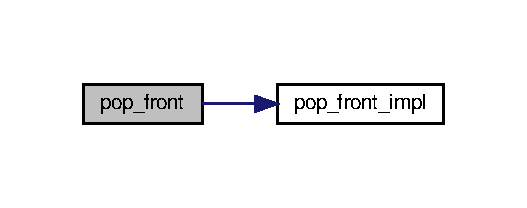
\includegraphics[width=253pt]{proxy_8hpp_a6ba8a69fe5dfb69975740463e80ce89b_cgraph}
\end{center}
\end{figure}
Here is the caller graph for this function\+:
\nopagebreak
\begin{figure}[H]
\begin{center}
\leavevmode
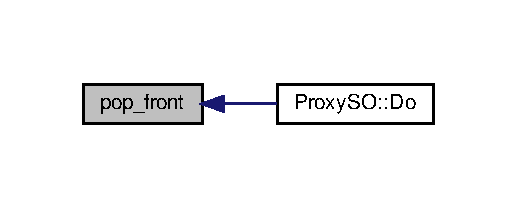
\includegraphics[width=248pt]{proxy_8hpp_a6ba8a69fe5dfb69975740463e80ce89b_icgraph}
\end{center}
\end{figure}
\mbox{\Hypertarget{proxy_8hpp_ae5e7ef9b08c7340386e7eccab535c7f0}\label{proxy_8hpp_ae5e7ef9b08c7340386e7eccab535c7f0}} 
\index{proxy.\+hpp@{proxy.\+hpp}!pop\+\_\+front\+\_\+impl@{pop\+\_\+front\+\_\+impl}}
\index{pop\+\_\+front\+\_\+impl@{pop\+\_\+front\+\_\+impl}!proxy.\+hpp@{proxy.\+hpp}}
\subsubsection{\texorpdfstring{pop\+\_\+front\+\_\+impl()}{pop\_front\_impl()}}
{\footnotesize\ttfamily template$<$typename Tuple , std\+::size\+\_\+t ... Is$>$ \\
auto pop\+\_\+front\+\_\+impl (\begin{DoxyParamCaption}\item[{const Tuple \&}]{tuple,  }\item[{std\+::index\+\_\+sequence$<$ Is... $>$}]{ }\end{DoxyParamCaption})}

Here is the caller graph for this function\+:
\nopagebreak
\begin{figure}[H]
\begin{center}
\leavevmode
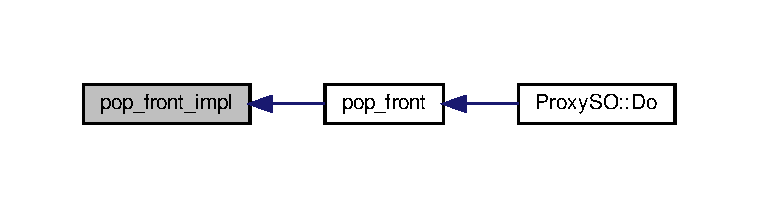
\includegraphics[width=350pt]{proxy_8hpp_ae5e7ef9b08c7340386e7eccab535c7f0_icgraph}
\end{center}
\end{figure}
\mbox{\Hypertarget{proxy_8hpp_a4f31a6fd48ee5d4579ae4aaaa3cae285}\label{proxy_8hpp_a4f31a6fd48ee5d4579ae4aaaa3cae285}} 
\index{proxy.\+hpp@{proxy.\+hpp}!sig\+\_\+handler@{sig\+\_\+handler}}
\index{sig\+\_\+handler@{sig\+\_\+handler}!proxy.\+hpp@{proxy.\+hpp}}
\subsubsection{\texorpdfstring{sig\+\_\+handler()}{sig\_handler()}}
{\footnotesize\ttfamily void sig\+\_\+handler (\begin{DoxyParamCaption}\item[{int}]{signo }\end{DoxyParamCaption})}

Here is the caller graph for this function\+:
\nopagebreak
\begin{figure}[H]
\begin{center}
\leavevmode
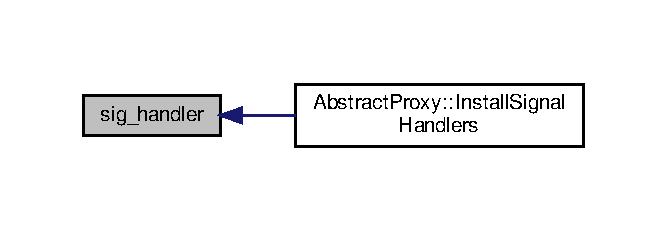
\includegraphics[width=320pt]{proxy_8hpp_a4f31a6fd48ee5d4579ae4aaaa3cae285_icgraph}
\end{center}
\end{figure}


\subsection{Variable Documentation}
\mbox{\Hypertarget{proxy_8hpp_a0fa3e25df0e6e54f52f9aea616c50d3b}\label{proxy_8hpp_a0fa3e25df0e6e54f52f9aea616c50d3b}} 
\index{proxy.\+hpp@{proxy.\+hpp}!child\+\_\+terminated@{child\+\_\+terminated}}
\index{child\+\_\+terminated@{child\+\_\+terminated}!proxy.\+hpp@{proxy.\+hpp}}
\subsubsection{\texorpdfstring{child\+\_\+terminated}{child\_terminated}}
{\footnotesize\ttfamily bool child\+\_\+terminated = false}

\mbox{\Hypertarget{proxy_8hpp_af735db148c9e9f49d4feb7a4f5271b7a}\label{proxy_8hpp_af735db148c9e9f49d4feb7a4f5271b7a}} 
\index{proxy.\+hpp@{proxy.\+hpp}!k\+Segment\+Magic@{k\+Segment\+Magic}}
\index{k\+Segment\+Magic@{k\+Segment\+Magic}!proxy.\+hpp@{proxy.\+hpp}}
\subsubsection{\texorpdfstring{k\+Segment\+Magic}{kSegmentMagic}}
{\footnotesize\ttfamily constexpr uint32\+\_\+t k\+Segment\+Magic = 0xc7390fbc}

\mbox{\Hypertarget{proxy_8hpp_a8b43c81ee7b8a4288c1cc31aad967e7d}\label{proxy_8hpp_a8b43c81ee7b8a4288c1cc31aad967e7d}} 
\index{proxy.\+hpp@{proxy.\+hpp}!k\+S\+H\+M\+Alignment@{k\+S\+H\+M\+Alignment}}
\index{k\+S\+H\+M\+Alignment@{k\+S\+H\+M\+Alignment}!proxy.\+hpp@{proxy.\+hpp}}
\subsubsection{\texorpdfstring{k\+S\+H\+M\+Alignment}{kSHMAlignment}}
{\footnotesize\ttfamily constexpr int k\+S\+H\+M\+Alignment = 8}

\mbox{\Hypertarget{proxy_8hpp_afc2f556ffb367cbd8559aa26d9baa913}\label{proxy_8hpp_afc2f556ffb367cbd8559aa26d9baa913}} 
\index{proxy.\+hpp@{proxy.\+hpp}!parent\+\_\+terminated@{parent\+\_\+terminated}}
\index{parent\+\_\+terminated@{parent\+\_\+terminated}!proxy.\+hpp@{proxy.\+hpp}}
\subsubsection{\texorpdfstring{parent\+\_\+terminated}{parent\_terminated}}
{\footnotesize\ttfamily bool parent\+\_\+terminated = false}


\hypertarget{libtest_8cpp}{}\section{tests/libtest.cpp File Reference}
\label{libtest_8cpp}\index{tests/libtest.\+cpp@{tests/libtest.\+cpp}}
{\ttfamily \#include $<$tuple$>$}\newline
Include dependency graph for libtest.\+cpp\+:
\nopagebreak
\begin{figure}[H]
\begin{center}
\leavevmode
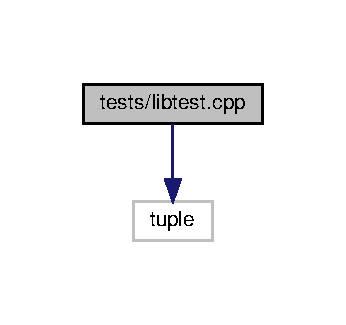
\includegraphics[width=166pt]{libtest_8cpp__incl}
\end{center}
\end{figure}
\subsection*{Functions}
\begin{DoxyCompactItemize}
\item 
int \hyperlink{libtest_8cpp_a90e4ba2b3b941b7dd2587d9770aa9ba7}{add} (std\+::tuple$<$ int, int $>$ tup)
\end{DoxyCompactItemize}


\subsection{Function Documentation}
\mbox{\Hypertarget{libtest_8cpp_a90e4ba2b3b941b7dd2587d9770aa9ba7}\label{libtest_8cpp_a90e4ba2b3b941b7dd2587d9770aa9ba7}} 
\index{libtest.\+cpp@{libtest.\+cpp}!add@{add}}
\index{add@{add}!libtest.\+cpp@{libtest.\+cpp}}
\subsubsection{\texorpdfstring{add()}{add()}}
{\footnotesize\ttfamily int add (\begin{DoxyParamCaption}\item[{std\+::tuple$<$ int, int $>$}]{tup }\end{DoxyParamCaption})}


\hypertarget{tests_8cpp}{}\section{tests/tests.cpp File Reference}
\label{tests_8cpp}\index{tests/tests.\+cpp@{tests/tests.\+cpp}}
{\ttfamily \#include $<$map$>$}\newline
{\ttfamily \#include $<$tuple$>$}\newline
{\ttfamily \#include $<$type\+\_\+traits$>$}\newline
{\ttfamily \#include $<$netinet/in.\+h$>$}\newline
{\ttfamily \#include $<$arpa/inet.\+h$>$}\newline
{\ttfamily \#include $<$dlfcn.\+h$>$}\newline
{\ttfamily \#include $<$gtest/gtest.\+h$>$}\newline
{\ttfamily \#include $<$proxy.\+hpp$>$}\newline
Include dependency graph for tests.\+cpp\+:
\nopagebreak
\begin{figure}[H]
\begin{center}
\leavevmode
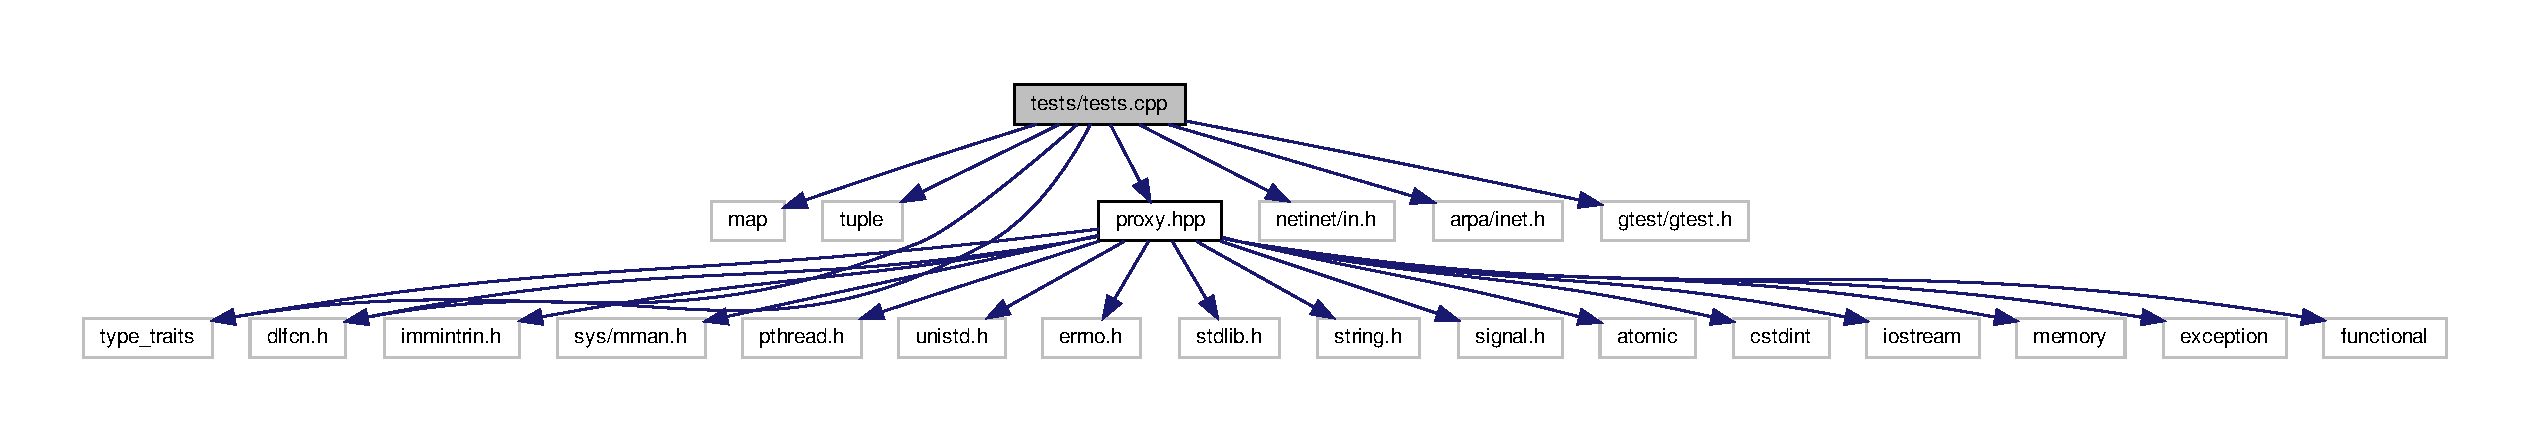
\includegraphics[width=350pt]{tests_8cpp__incl}
\end{center}
\end{figure}
\subsection*{Macros}
\begin{DoxyCompactItemize}
\item 
\#define \hyperlink{tests_8cpp_a22caf0152144d7bd7533555a70dd616f}{\+\_\+}(n)~std\+::get$<$n$>$(tup)
\item 
\#define \hyperlink{tests_8cpp_ab18ca25ea5500baf22b6fc41db84ad44}{\+\_\+res}~\hyperlink{tests_8cpp_a22caf0152144d7bd7533555a70dd616f}{\+\_\+}(0)
\end{DoxyCompactItemize}


\subsection{Macro Definition Documentation}
\mbox{\Hypertarget{tests_8cpp_a22caf0152144d7bd7533555a70dd616f}\label{tests_8cpp_a22caf0152144d7bd7533555a70dd616f}} 
\index{tests.\+cpp@{tests.\+cpp}!\+\_\+@{\+\_\+}}
\index{\+\_\+@{\+\_\+}!tests.\+cpp@{tests.\+cpp}}
\subsubsection{\texorpdfstring{\+\_\+}{\_}}
{\footnotesize\ttfamily \#define \+\_\+(\begin{DoxyParamCaption}\item[{}]{n }\end{DoxyParamCaption})~std\+::get$<$n$>$(tup)}

\mbox{\Hypertarget{tests_8cpp_ab18ca25ea5500baf22b6fc41db84ad44}\label{tests_8cpp_ab18ca25ea5500baf22b6fc41db84ad44}} 
\index{tests.\+cpp@{tests.\+cpp}!\+\_\+res@{\+\_\+res}}
\index{\+\_\+res@{\+\_\+res}!tests.\+cpp@{tests.\+cpp}}
\subsubsection{\texorpdfstring{\+\_\+res}{\_res}}
{\footnotesize\ttfamily \#define \+\_\+res~\hyperlink{tests_8cpp_a22caf0152144d7bd7533555a70dd616f}{\+\_\+}(0)}


%--- End generated contents ---

% Index
\backmatter
\newpage
\phantomsection
\clearemptydoublepage
\addcontentsline{toc}{chapter}{Index}
\printindex

\end{document}
